\documentclass{beamer}
\usetheme{Madrid}
%\usepackage[orientation=landscape,size=custom,width=28,height=21,scale=1,debug]{beamerposter} 
% width=11.333,height=8.5
\geometry{paperwidth=8.5in,paperheight=4.75in} 
% paperwidth=11.333in,paperheight=8.5in

%	%%%%%%%%%%%%%	%
% Load packages %
%	%%%%%%%%%%%%%	%

%\usepackage{helvet}
%\usepackage{tikz}
%\usepackage{lmodern} % Load Latin Modern fonts
%\usepackage{subcaption}
%\usepackage{multirow}
\usepackage{booktabs} % For better table rules
%\usepackage{graphicx} % for including graphics
%\usepackage{multicol}
%\usepackage{amsmath}
\usepackage[citestyle=authoryear, bibstyle=authoryear, sorting=nyt]{biblatex}
\AtEveryBibitem{
	\clearfield{issn}
	\ifentrytype{book}{\clearfield{isbn}}{}
    \clearfield{urlyear}
    \clearfield{urlmonth}
    \clearfield{urlday}
}
\addbibresource{../ps_honors_thesis.bib}

%----- Beamer options -----%
\AtBeginSection[]
{
  \begin{frame}
    \frametitle{Table of Contents}
    \tableofcontents[currentsection]
  \end{frame}
}

\setbeameroption{hide notes} % Only slides
%\setbeameroption{show only notes} % Only notes
%\setbeameroption{show notes on second screen=right} % Both
\setbeamertemplate{navigation symbols}{} % No navigation buttons

\setbeamercolor{frametitle}{bg=cyan!7, fg=black}

% Redefine bibliography colors to black
\setbeamercolor{bibliography entry author}{fg=black}
\setbeamercolor{bibliography entry title}{fg=black} % Set book titles to black
\setbeamercolor{bibliography entry note}{fg=black}
\setbeamercolor{caption name}{fg=black}
\setbeamercolor{title}{bg=cyan!7, fg=black}
\setbeamercolor{subtitle}{bg=white, fg=black}

\setbeamerfont{bibliography entry author}{size=\small}
\setbeamerfont{bibliography entry title}{size=\small}
\setbeamerfont{bibliography entry note}{size=\small}
\setbeamerfont{caption name}{size=\small}

\title{The Policing of the “Reserve Army”}
\subtitle{Economic Inequality and Police Killings}
\author{Matthew A. Carson}\date{May 21, 2024}

\begin{document}

\begin{frame}
  \titlepage
  \note[item]{Welcome to the talk!}
\end{frame}

\section{Research Question and Design}
%----- Research Question -----%
\begin{frame}{Research Question}
	\begin{itemize}
		\item How does class, economic inequality, and gentrification contribute to the incidence of police killings in the US? \pause
		\note<1>{My research question is: How does class, economic inequality, and gentrification contribute to the incidence of police killings in the US?}
		\begin{itemize}
			\item There are sharp racial disparities.
			\item But what are the economic dimensions? \pause
			\note<2>[item]{There are sharp racial disparities.}
			\note<2>[item]{But what are the economic dimensions?}
			\begin{itemize}
				\item I'm interested specifically in looking at place. \pause
				\note<3>[item]{I'm interested specifically in looking at place.}
			\end{itemize}
			\item How do processes of gentrification contribute to rates of police killings?
			\note<4>[item]{And how processes of gentrification contribute to rates of police killings}
		\end{itemize}		
	\end{itemize}
\end{frame}

%----- Research Design -----%
\begin{frame}{Research Design: Data Sources}
	\begin{itemize}
	\item US Census American Community Survey
		\begin{itemize}
			\item Median Family Income in tracts
			\item Racial composition of tracts
		\end{itemize} \pause
	\item FatalEncounters.org
		\begin{itemize}
			\item List of people killed by law enforcement in the US
			\item Compiled by journalists -- FBI data not reliable
			\item Includes latitude and longitude
			\item Years in this study 2015--2020, inclusive
		\end{itemize} \pause
	\item Urban Displacement Project Typologies \nocite{udpDisplacementGentrificationTypologies2023}
		\begin{itemize}
			\item Condensed into three typologies
			\begin{itemize}
				\item Low-Income or At-Risk
				\item Gentrifying
				\item Stable
			\end{itemize}
		\end{itemize}
	\end{itemize}
	\note<1>{
	I used the US Census's American Community Survey to obtain median family income for US census tracts and the racial composition of each tract.}
	\note<2>{
	\begin{itemize}
	\item I obtained a list of police killings of lethal uses of force from Fatal Ecnounters [dot] org.
	\item Journalists have compiled a list of people killed by law enforcement from local news reports.
	\item Using the latitude and longitude, I matched the police killing with the census tract data set.
	\item I used years 2015--2020 for the study.
	\end{itemize}
	}
	\note<3>{
	For gentrification, I used the typologies from the Urban Displacement Project.\newline\newline
	I condensed their nine typologies into three:
		\begin{itemize}
			\item Low-Income or At-Risk
			\item Gentrifying
			\item Stable
		\end{itemize}
		}
\end{frame}

\begin{frame}{Research Design: Definitions}
	\begin{itemize}
		\item Lethal Use of Force (LUOF)
		\begin{itemize}
			\item Include: Level of Force Applied
			\begin{itemize}
				\item  tasered, gunshot, stabbed, asphyxiated/restrained, beaten/bludgeoned with an instrument, chemical agent/pepper spray, asphyxiation/restrained, or less than lethal force.
			\end{itemize}
			\item Exclude: Cause
			\begin{itemize}
				\item vehicle, fell from a height, drowned, medical emergency, other, burned/smoke inhalation, drug overdose, and undetermined.
			\end{itemize}
		\end{itemize}
	\end{itemize}
	\note[item]{Fatal Encounters [dot] org cases where the level of force applied was categorized as: \textbf{tasered, gunshot, stabbed, asphyxiated/restrained, beaten/bludgeoned with an instrument, chemical agent/pepper spray, asphyxiation/restrained, or less than lethal force} were included.}
	\note[item]{An important note: all cases resulted in a death; those classified as "less than lethal force" were cases where a "less than lethal" intervention technique resulted in a death.}
	\note[item]{I excluded the following causes of death: \textbf{vehicle, fell from a height, drowned, medical emergency, other, burned/smoke inhalation, drug overdose, and undetermined.}}
\end{frame}

\begin{frame}{Research Design: Gentrification}
\begin{center}
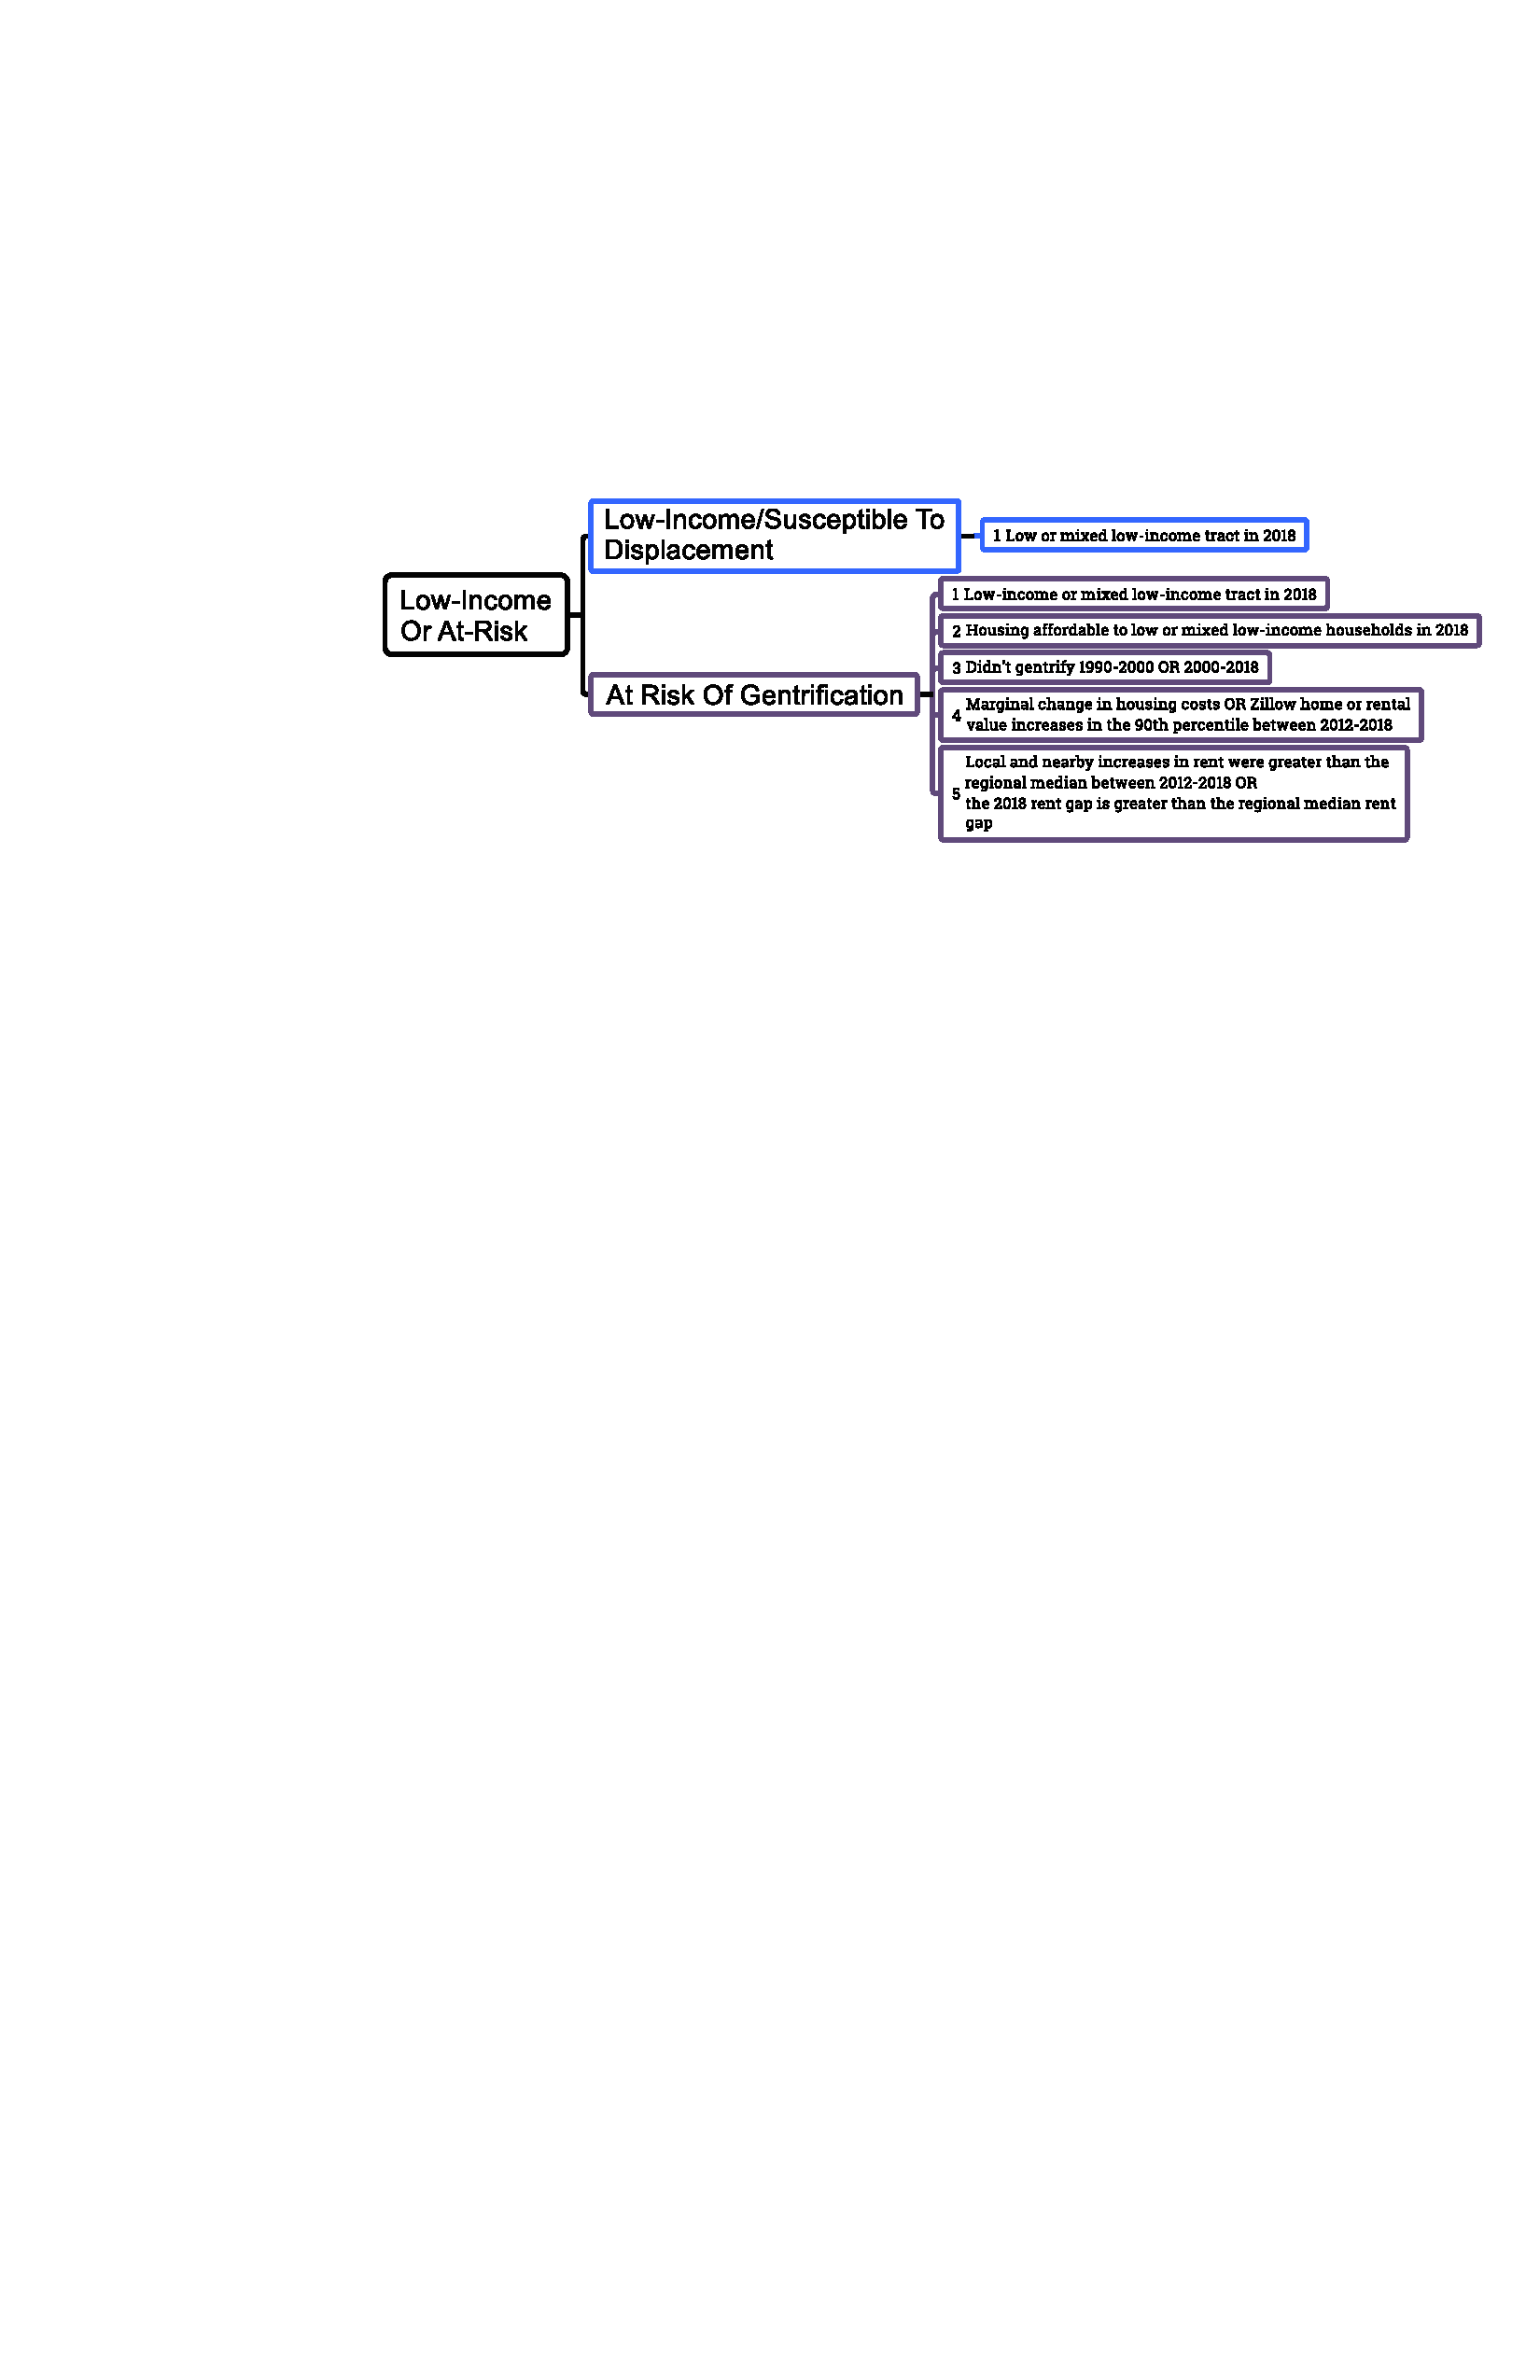
\includegraphics[scale=1]{images/low_income_at_risk}
\end{center}
\note[item]{Because the Urban Displacement Project had so many displacement typologies, I combined them into three.}
\note[item]{The typologies — “low-income/susceptible to displacement” and “at risk of gentrification” — have been merged into “low-income or at-risk”; this combines tracts that are low or mixed-low income and tracts that are at risk of gentrification because of rent increases in nearby tracts—referred to as a rent gap—but excludes tracts that are gentrifying.}
\end{frame}

\begin{frame}{Research Design: Gentrification}
\begin{center}
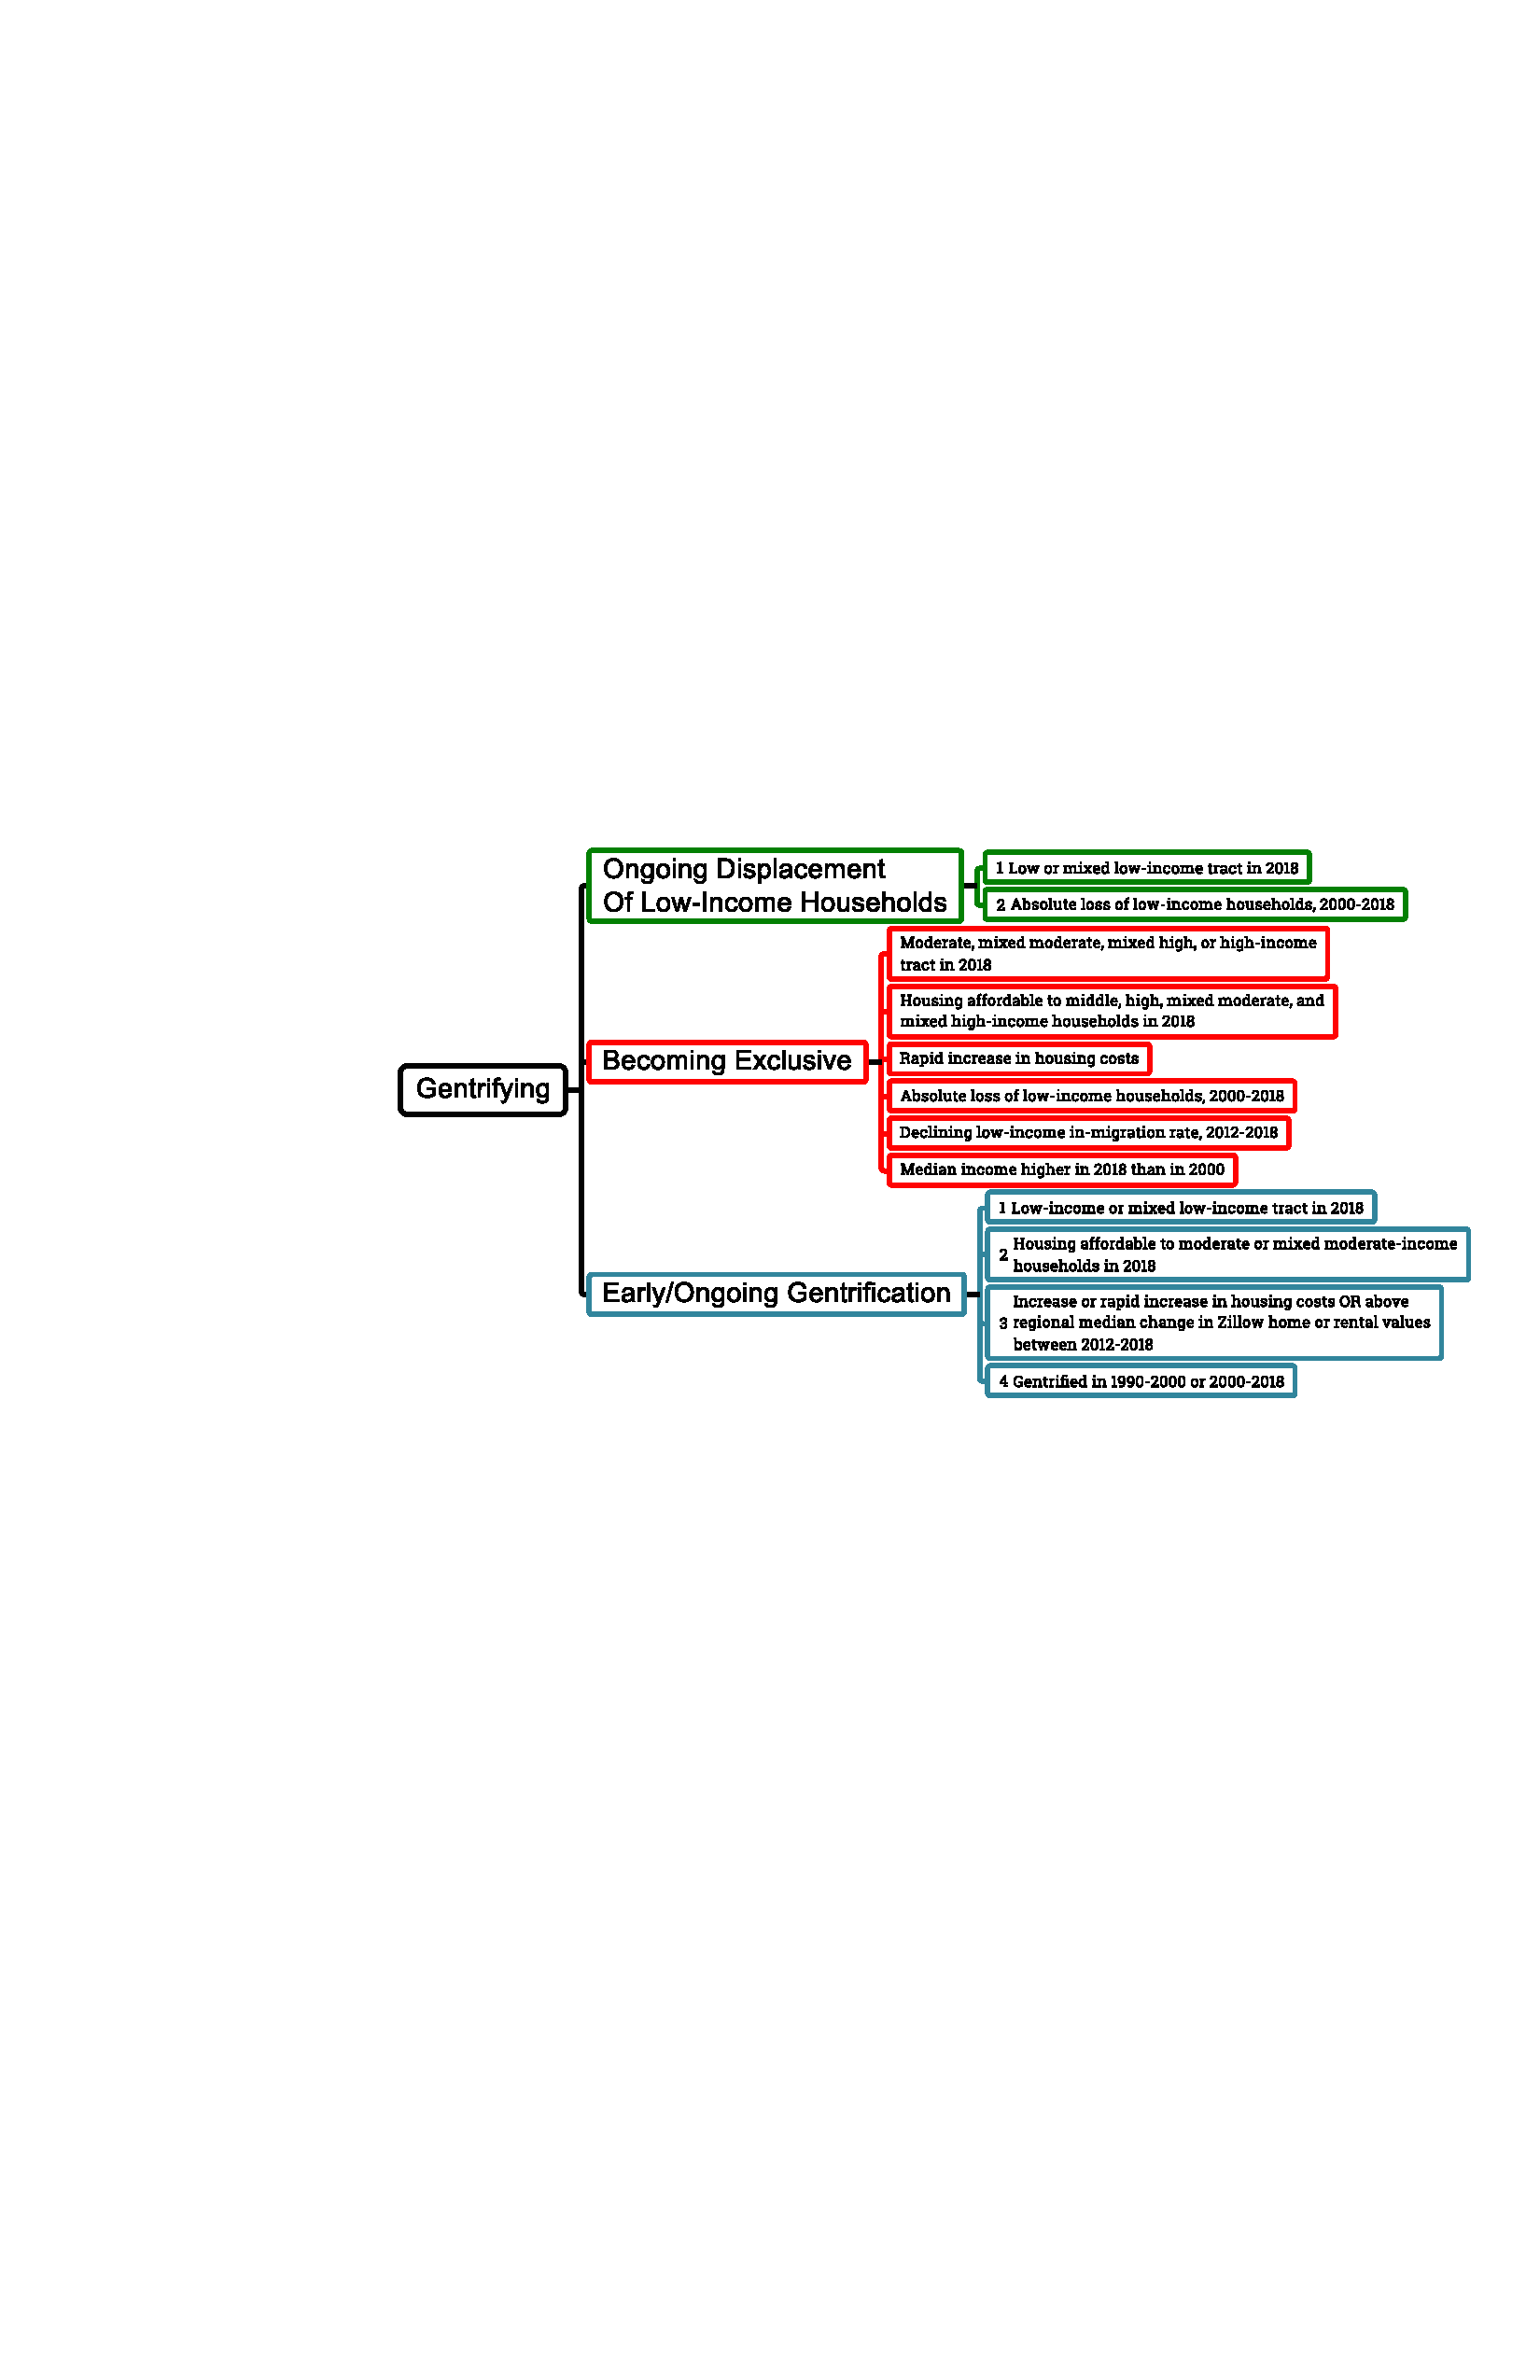
\includegraphics[scale=1]{images/gentrifying}
\end{center}
\note[item]{Next, all typologies where tracts are gentrifying or residents are being displaced were combined into “gentrifying”; this includes “ongoing displacement of low-income households,” “early/ongoing gentrification” and “becoming exclusive.”}
\end{frame}

\begin{frame}{Research Design: Gentrification}
\begin{center}
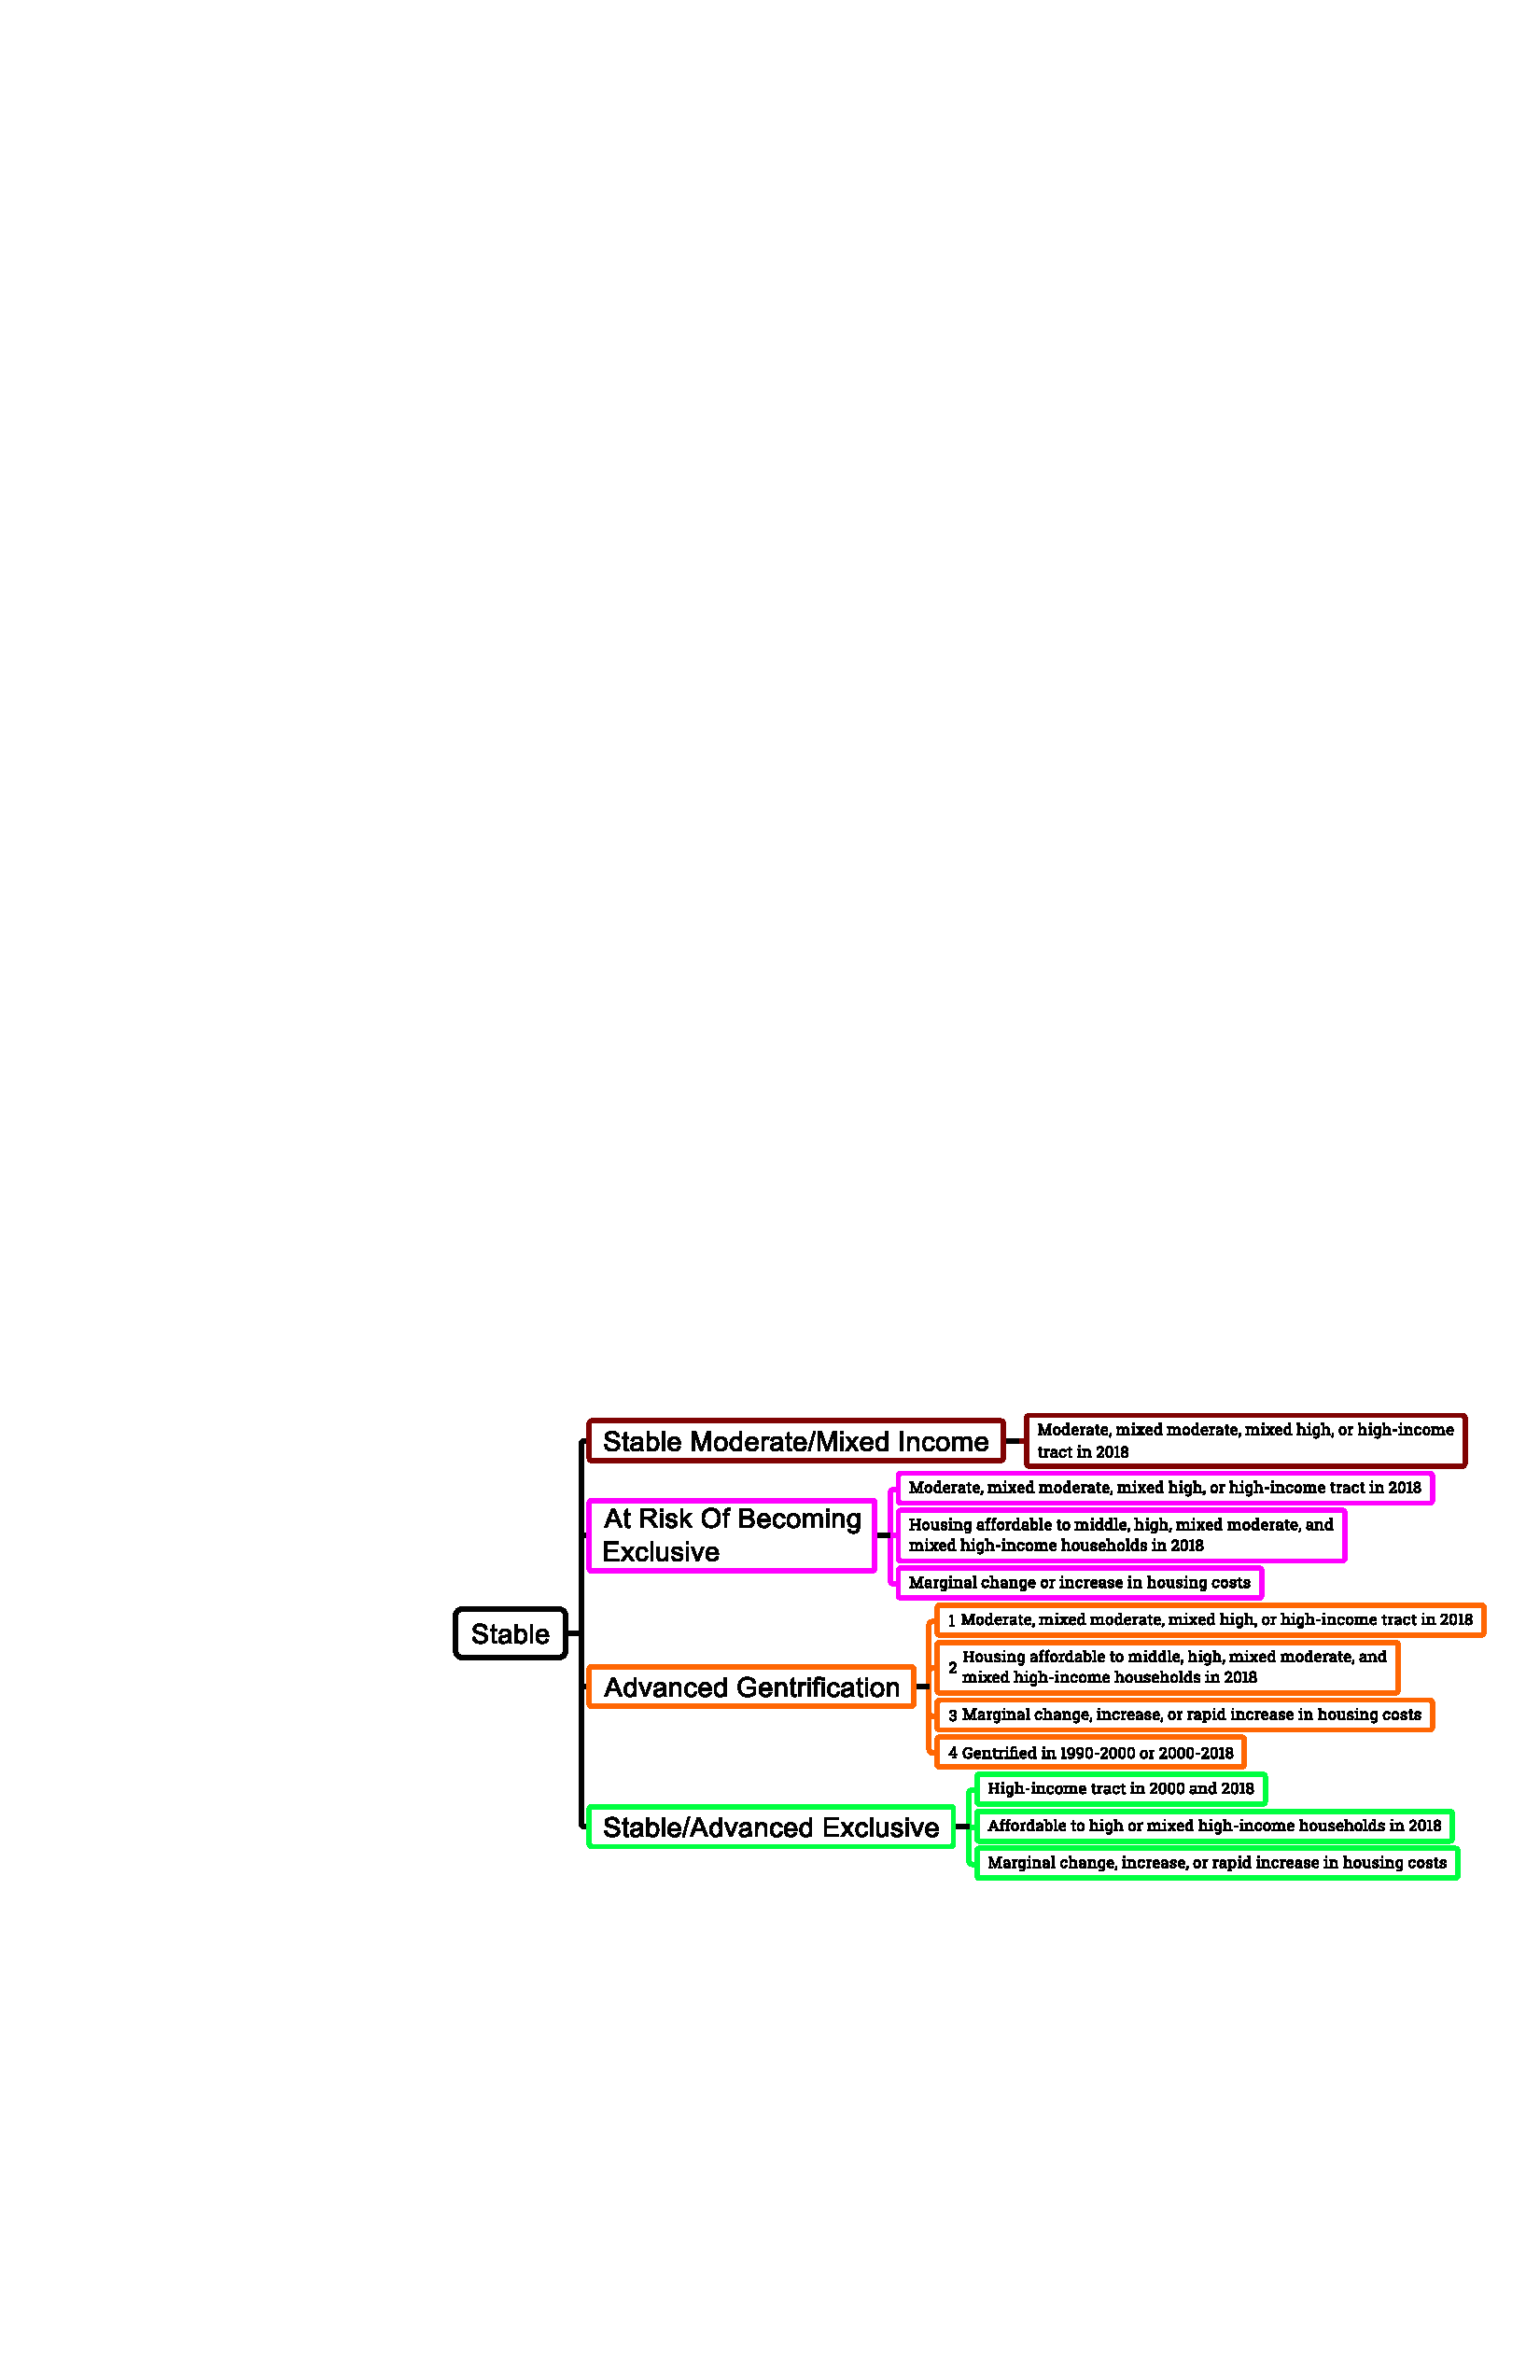
\includegraphics[scale=1]{images/stable}
\end{center}
\note[item]{The last group includes those tracts that are either stable in terms of income or housing costs or both, including those tracts that have already gentrified either in 1990 or 2000: “stable moderate/mixed-income,” “at risk of becoming exclusive,” “advanced gentrification,” “stable/advanced exclusive.” They are combined into the category “stable”}
\note[item]{The reason for including stable census tracts and advanced gentrification tracts in the same category is that the latter have already been gentrified before the period that this study is examining and thus would not be appropriate for inclusion in the category where gentrification is occurring.}
\end{frame}

\begin{frame}{Research Design: Hypotheses}
	\begin{tabular}{@{} l @{\hspace{18pt}} p{432pt} @{}}
	$\textbf{H}_1$: & LUOF rates should vary more substantially by income quintiles within each racial group than by racial groups within each income quintile. The lowest income quintiles should have the highest LUOF rates.
	\end{tabular} \pause
	\vfill
	\begin{tabular}{@{} l @{\hspace{18pt}} p{432pt} @{}}
	$\textbf{H}_2$: &Tracts experiencing gentrification or vulnerable to becoming gentrified should experience higher rates of LUOF than tracts that are not experiencing gentrification, regardless of the racial composition of the tract.
	\end{tabular}
	\note<1>[item]{I had two hypothses.}
	\note<1>[item]{The first one: LUOF rates would vary more substantially by income quintiles within each racial group than by racial groups within each income quintile. The lowest income quintiles should have the highest LUOF rates.}
	\note<2>{The second hypothesis is: Tracts experiencing gentrification or vulnerable to becoming gentrified should experience higher rates of LUOF than tracts that are not experiencing gentrification, regardless of the racial composition of the tract.}
\end{frame}

\section{Literature Review}
%---- Literature Review ------%
\begin{frame}{Literature Review}
	\begin{itemize}
		\item Johnson \parencites*{
		johnsonAfterwordBaltimorePolicing2016, 
		johnsonTrumpismPolicingProblem2019, 
		johnsonBlackLivesMatter2023}
		\item \textcite{wacquantClassRaceHyperincarceration2010}
		\item \textcite{feldmanPoliceKillingsUS2020, feldmanPoliceRelatedDeathsNeighborhood2019}
	\end{itemize}
\end{frame}

%----- Findings -----%
\section{Findings: Race and Tract Income}
\begin{frame}{Findings: Rates by Race/Ethnicity}
	\begin{center}
	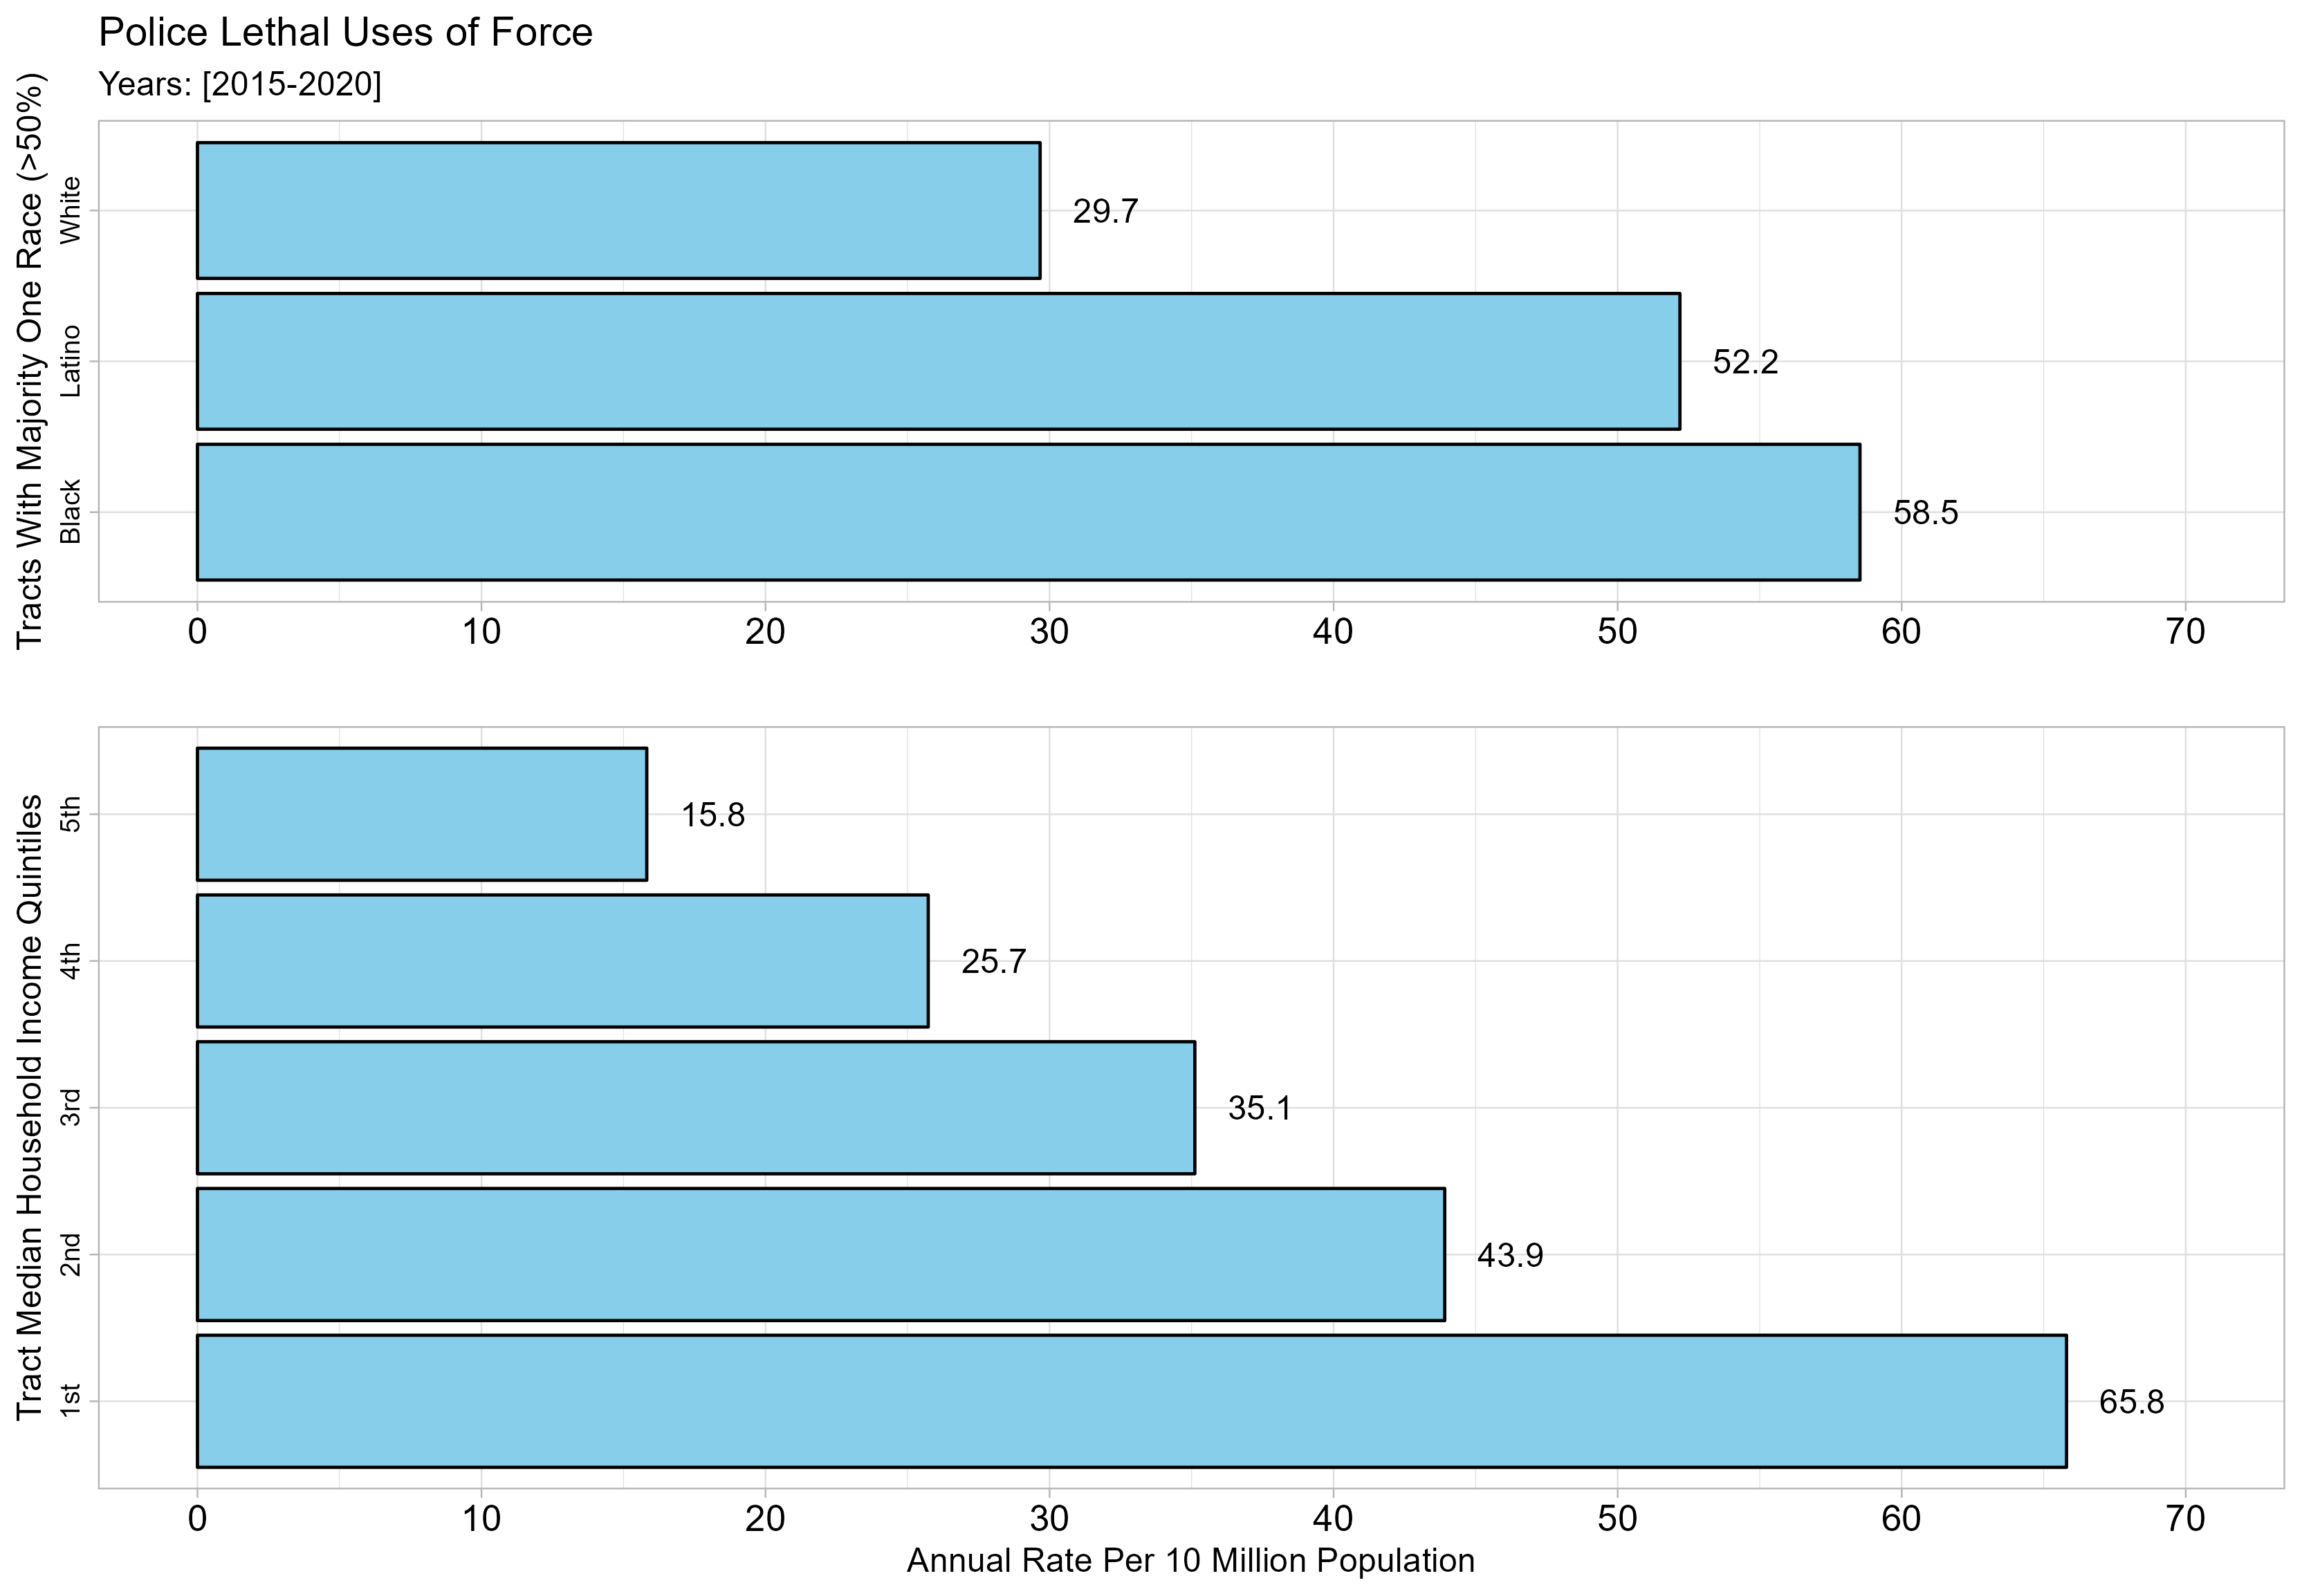
\includegraphics[height=0.8\textheight]{images/combined}	
	\end{center}
	\note[item]{Majority-black neighborho ods experience a rate nearly twice that of majority-white neighborhoods.}
	\note[item]{Majority-Hispanic/Latino neighborhoods experience a rate 1.75 times greater than majority-white neighborhoods.}
	\note[item]{US census tracts were binned into quintiles based on the distribution of median household income across all US census tracts.}
	\note[item]{Median household income has a strong relationship with the rate of police killings.}
	\note[item]{Police killings occur at the greatest frequency in the lowest-income tracts.}
	\note[item]{The lowest household income quintile tracts experience a rate over four times that of the highest household income tracts.}
%	\vspace*{24pt}
\end{frame}

%\begin{frame}{Findings: Median Household Income}
%	\begin{center}
%	\includegraphics[width=0.5\linewidth]{images/income_quintiles_only}
%	\end{center}
%	\vspace*{24pt}
%\end{frame}

\begin{frame}{Findings: Median Household Income}
	\begin{center}
		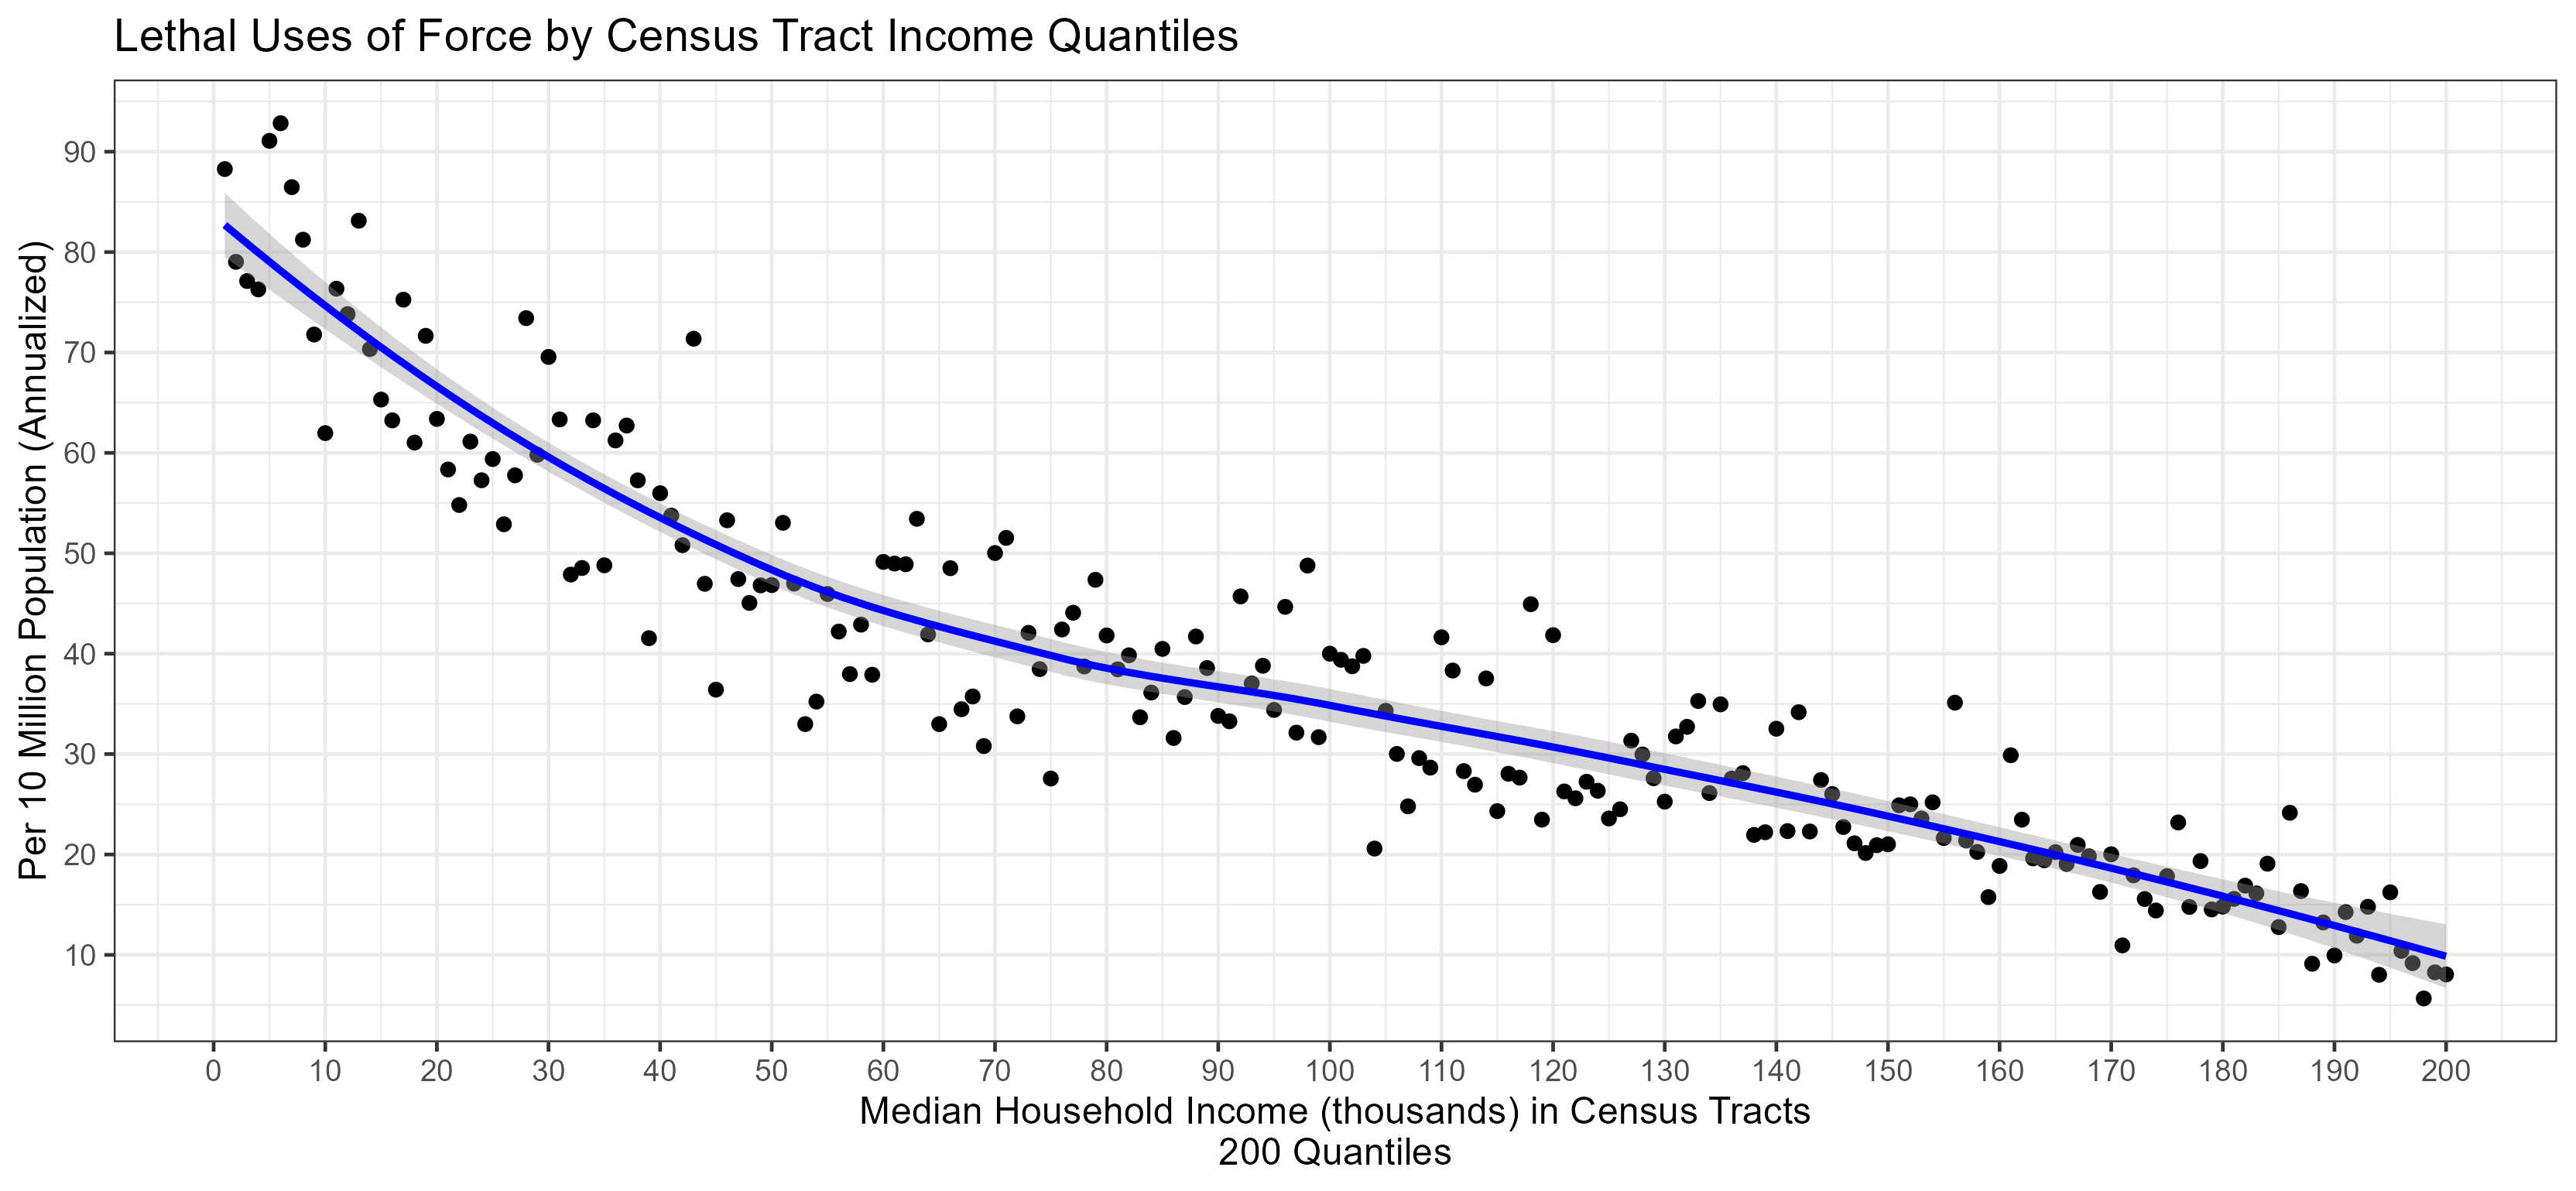
\includegraphics[width=\linewidth]{images/all_200}
	\end{center}
	\note{Another more granular income quantile approach shows a bit more variation by household income but is consistent with the bar plot and quintile analysis. By dividing tracts into two hundred quantiles with roughly the same number of observations in each bin (i.e., a quantile twice as granular as a percentile where the first bin is the lowest 0.5 percentile), one observes a curvilinear relationship between household income and the annualized rate of LUOFs. The lowest income tracts experience the highest rate. The rate drops off somewhat quickly as income increases along the x-axis, but around the 50th quantile, the slope becomes more gradual.}
\end{frame}

\begin{frame}{Findings: Majority Race and Income}
	\begin{center}
		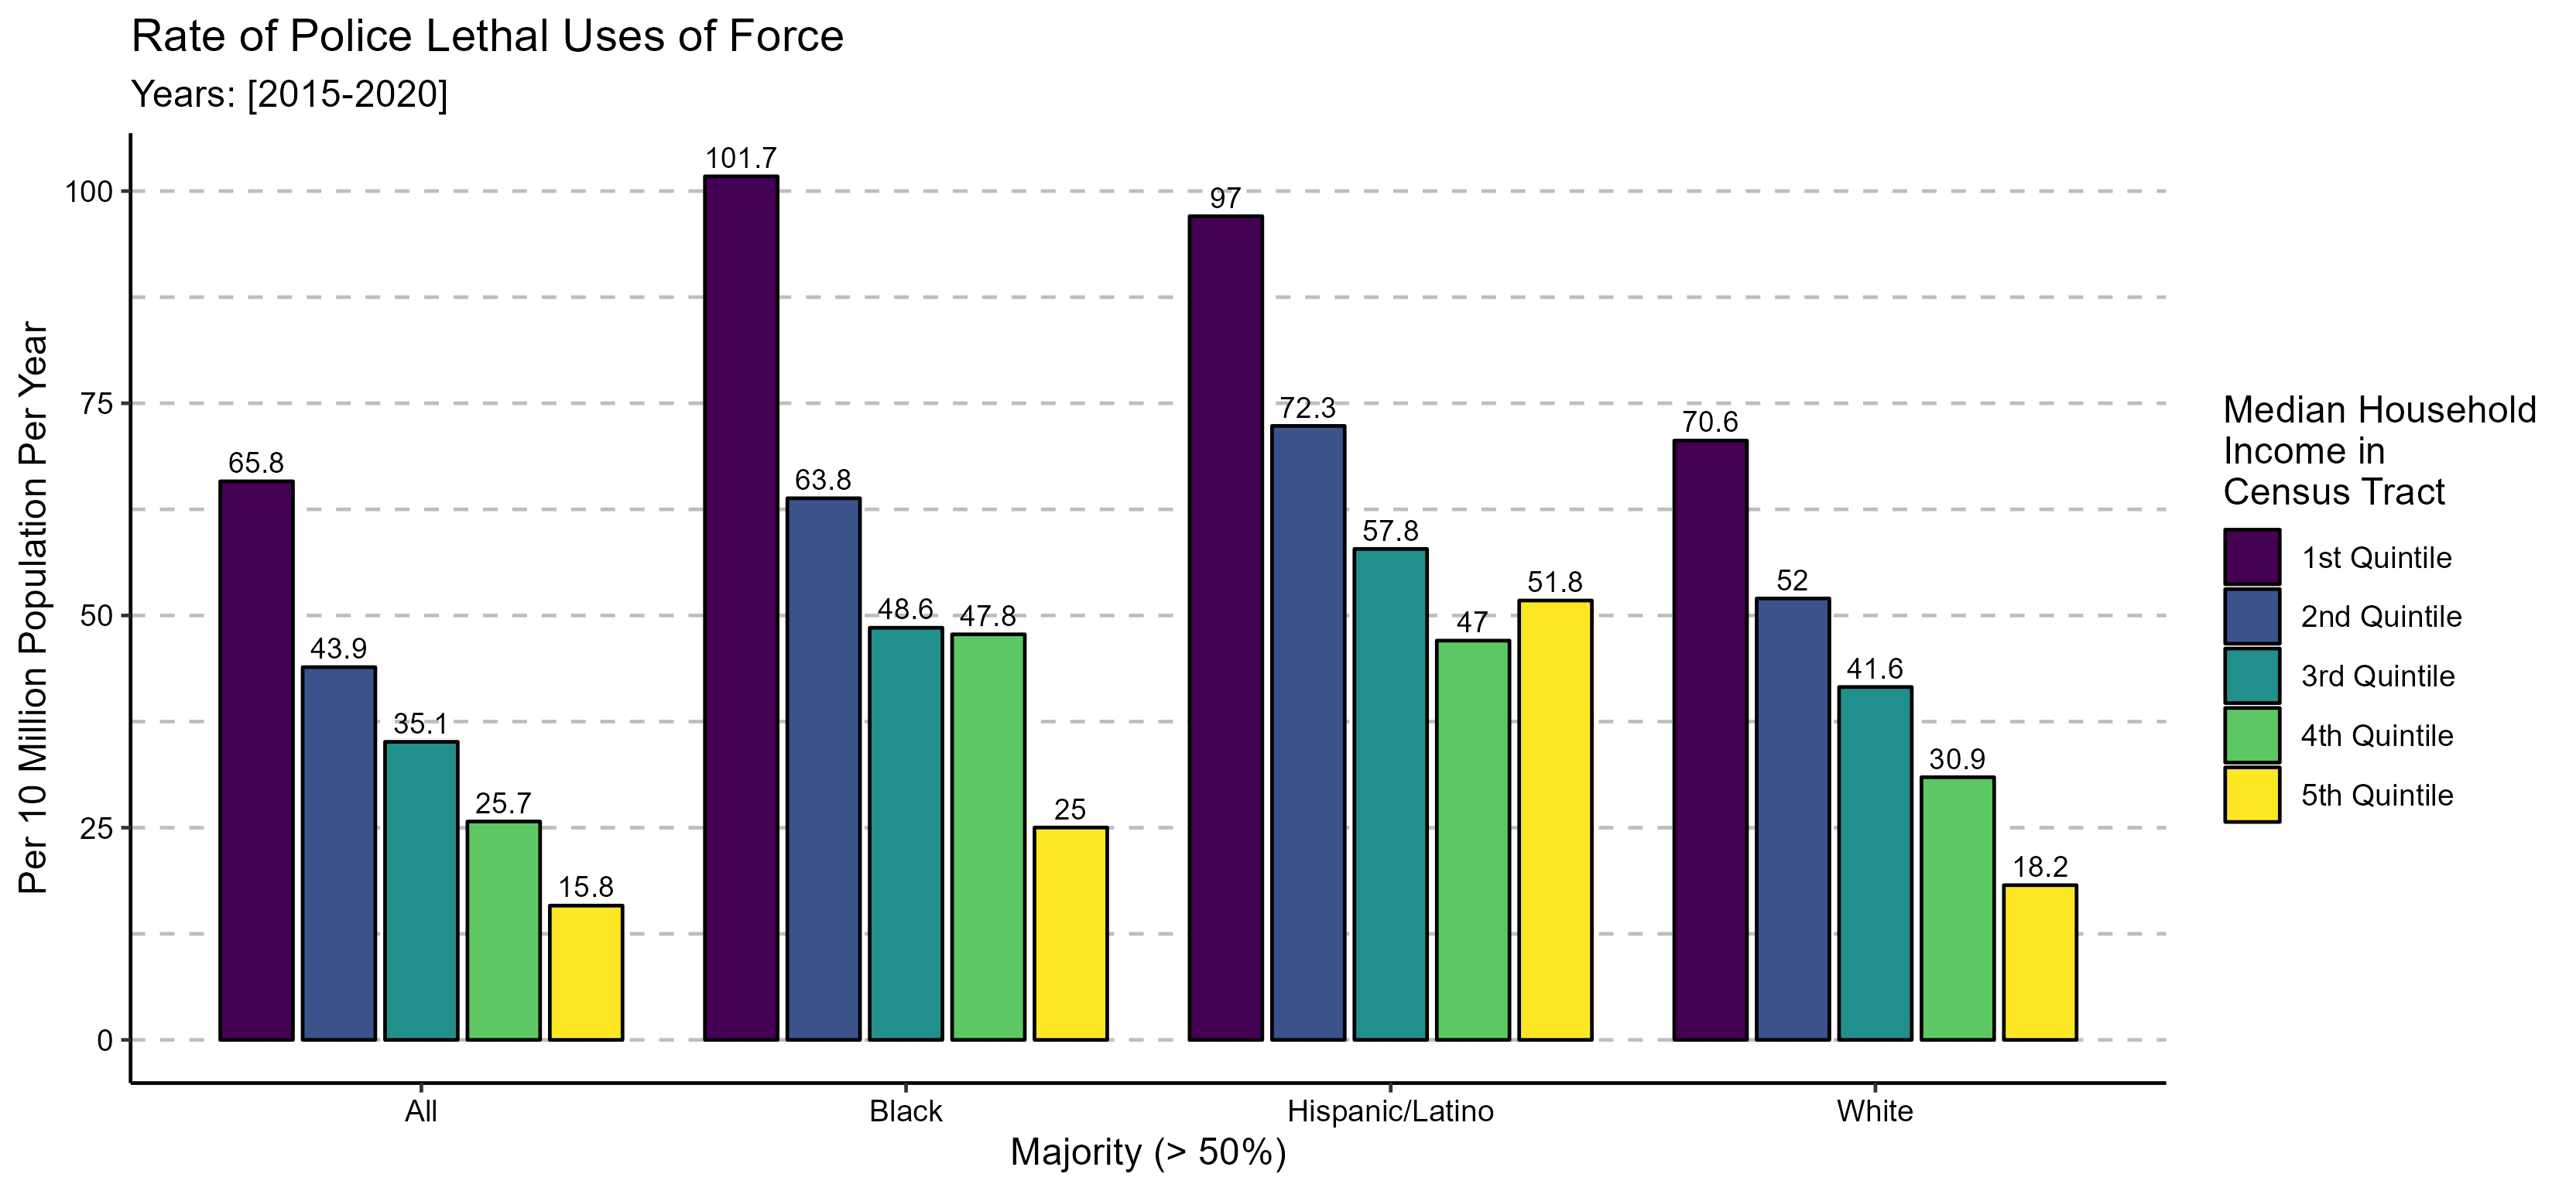
\includegraphics[width=\linewidth]{images/race_only_denom_race}
	\end{center}
	\note[item]{This figure shows the interactions between income and race.}
	\note[item]{The general trend of the lowest income quintiles experiencing the highest rates of LUOFs holds.}
	\note[item]{There is substantial variation by income quintile within racial and ethnic groups.}
	\note[item]{For all racial and ethnic groups, the lowest income quintile had the greatest lethal use of force rate.}
	\note[item]{The difference in the rate between the first and second quintile is substantial for majority black and Latino census tracts.}
\end{frame}

\begin{frame}{Logistic Regression: Income Only}
    \begin{columns}
    		% First column for the table
        \begin{column}{0.6\textwidth}
            \centering
            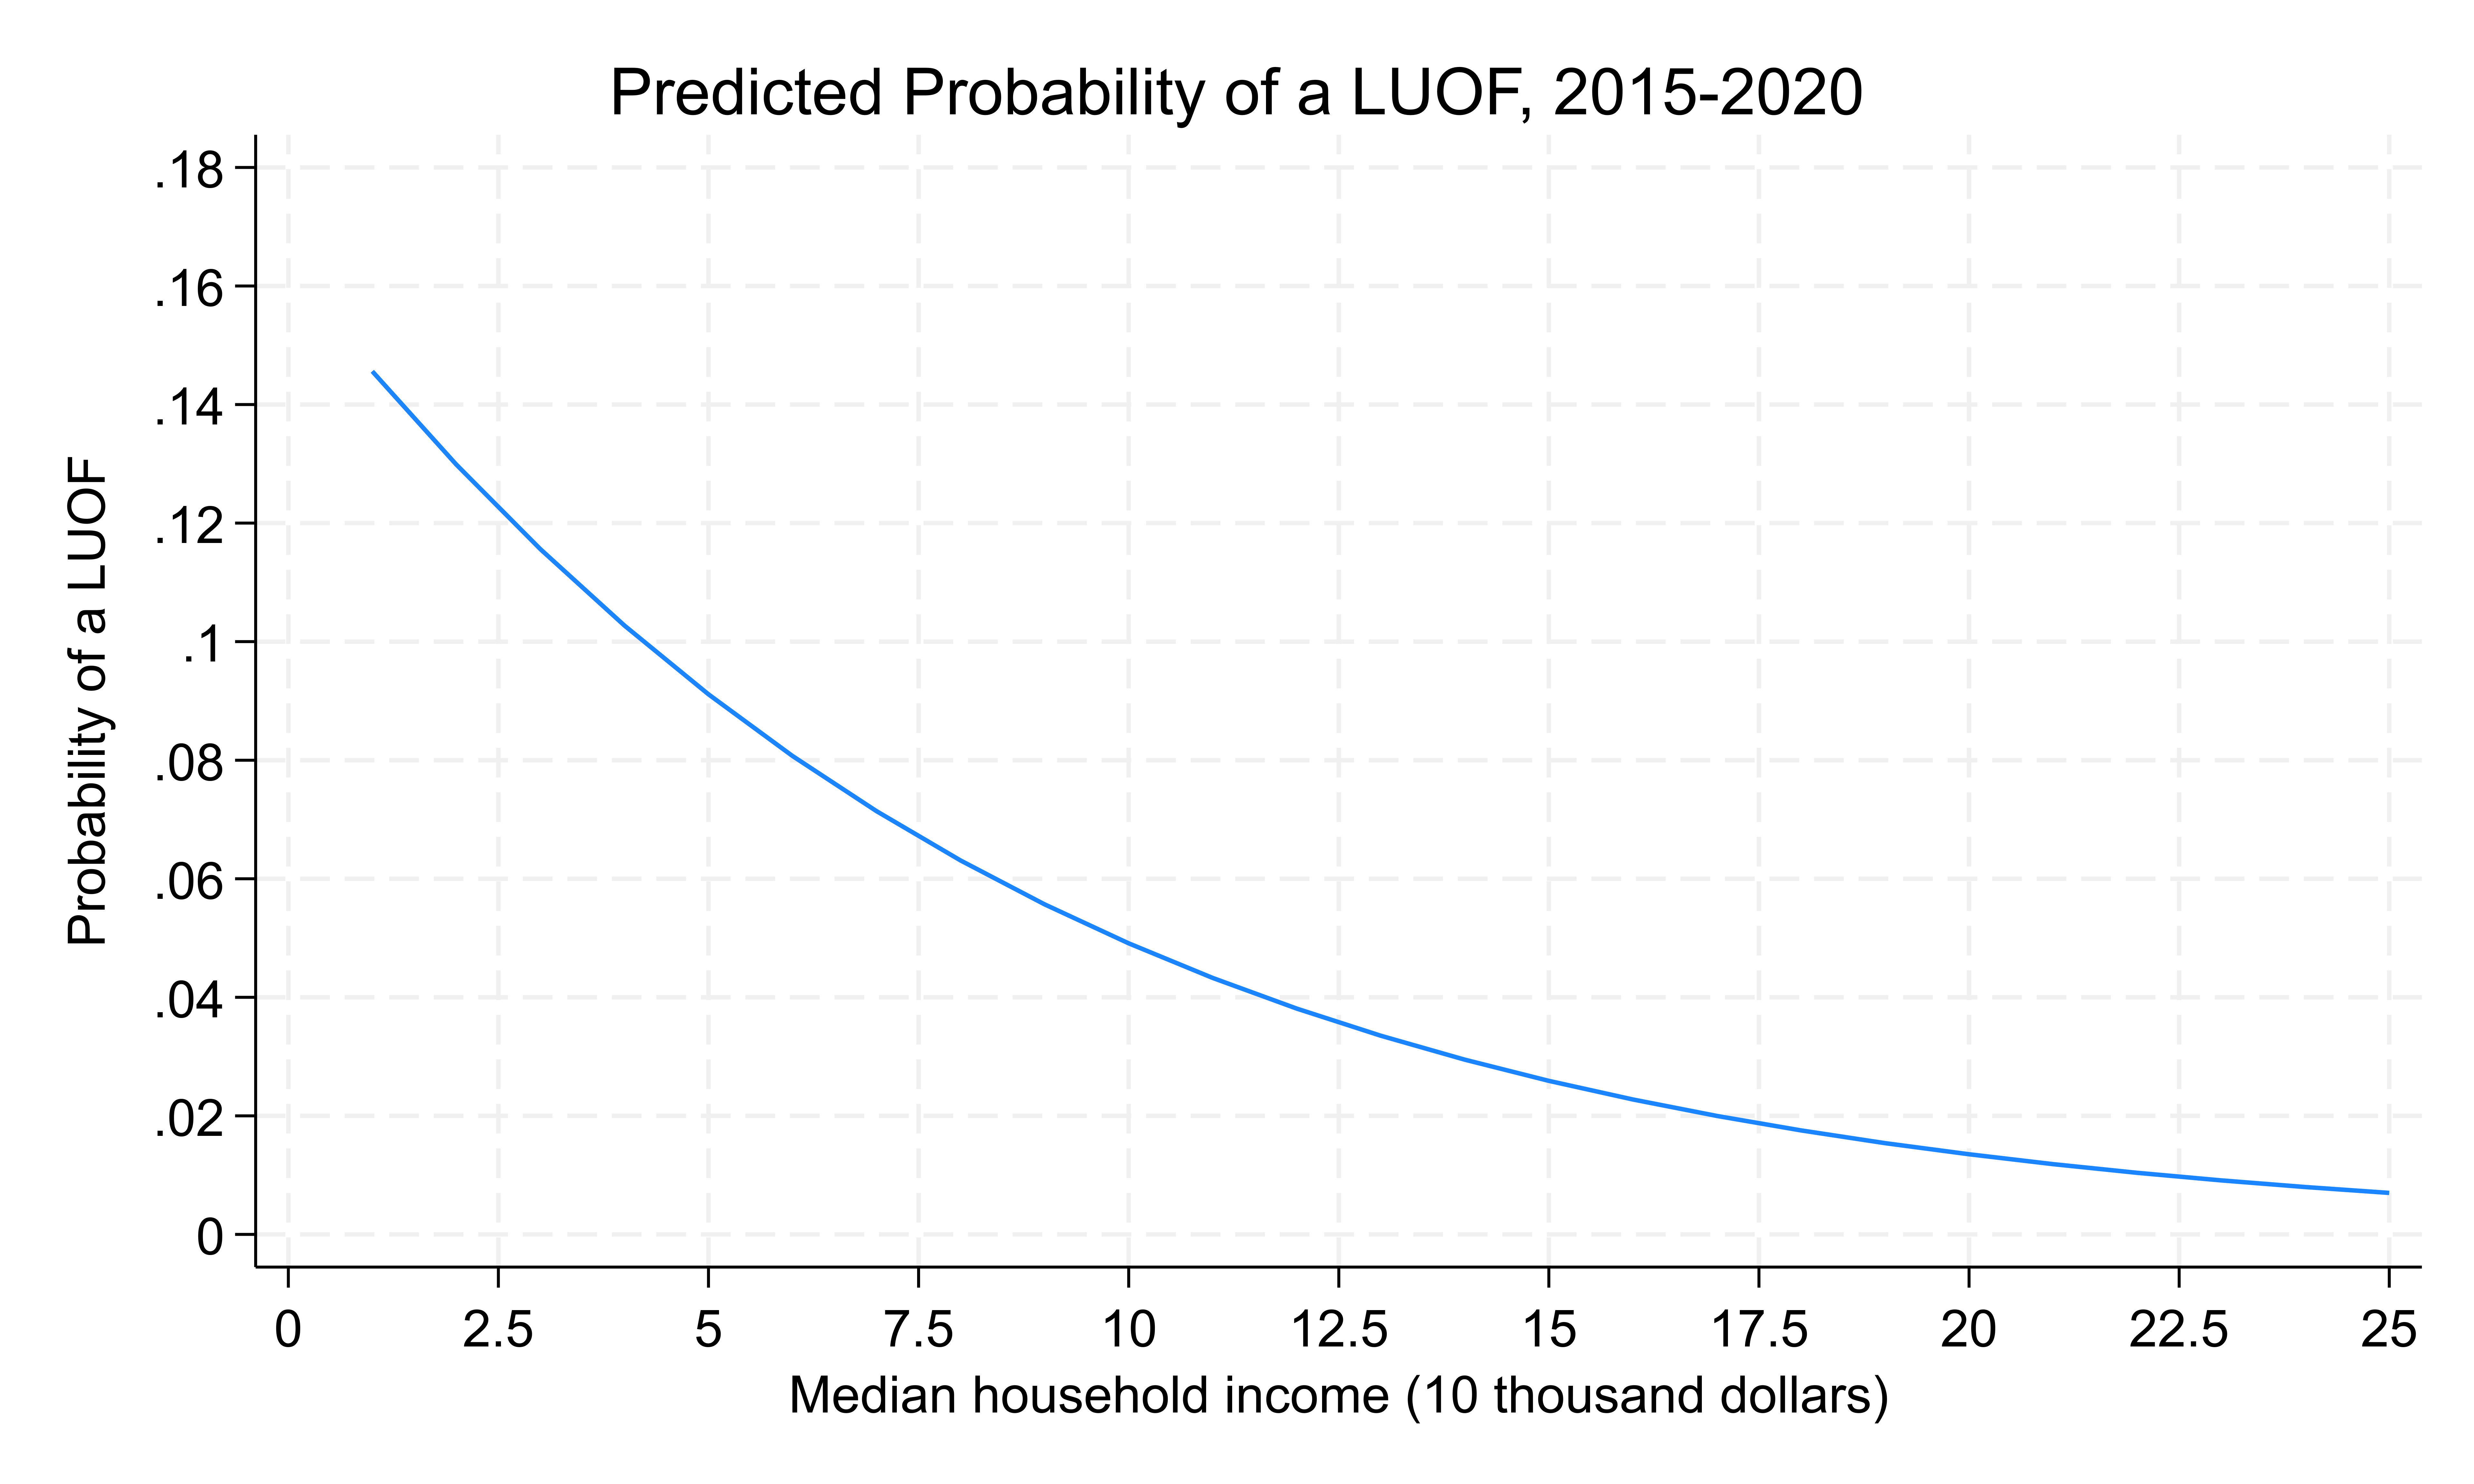
\includegraphics[width=\linewidth]{images/LUOF_logit_income_only}
        \end{column}
        % Second column for the image
        \begin{column}{0.4\textwidth}
        	\resizebox{\linewidth}{!}{%
                \begin{tabular}{lcccccc}
                    \toprule
                    Log likelihood: & -21947.515 & &Dependent Var: & LUOF $\ge1$ & & \\
                    \midrule
                    \multicolumn{3}{l}{Number of obs: 82,907} & \multicolumn{4}{l}{LR chi2(1): 875.58} \\
                    \multicolumn{3}{l}{Prob $>$ chi2: 0.0000} & \multicolumn{4}{l}{Pseudo R2: 0.0196} \\
                    \midrule
                    \midrule
                    Term & Coefficient & Std. err. & z & P$>|$z$|$ & \multicolumn{2}{c}{[95\% conf. interval]} \\
                    \midrule
                    Income (10k) & -0.1326502 & 0.0048988 & -27.08 & 0.000 & -0.1422516 & -0.1230488 \\
                    Intercept & -1.636736 & 0.0319747 & -51.19 & 0.000 & -1.699406 & -1.574067 \\
                    \bottomrule
                \end{tabular}
			} \pause
			
			\vspace{20pt}		
			
			$e^{-0.1326502} = 0.8758$
			
			\vspace{20pt}	
			
			$0.8758 - 1 = -0.1242$
			
			\vspace{20pt}	
			
			For every \$10k in income $\rightarrow 12.42$\% decrease in the odds of a census tract experiencing at least one LUOF.
        \end{column}
    \end{columns}
    \note<1>[item]{Next I constructed a logistic regression.}
    \note<1>[item]{The model estimates the odds of a census tract experiencing at least one LUOF based on the median household income of the census tract.}
    \note<1>[item]{I found a negative relationship between income and the odds of a tract experiencing at least one LUOF.}
    \note<2>[item]{If we exponentiate the coefficient for Income (10k) and subtract 1, we can estimate that for every ten thousand dollars in income, the odds of the tract experiencing at least one LUOF is 12.42 percent less.
    }
\end{frame}

\begin{frame}{Logistic Regressions: Race/Ethnicity}
%	\includegraphics[height=0.85\textheight]{images/LUOF_logit_bivariate}
    \begin{columns}
    		% First column for the table
        \begin{column}{0.6\textwidth}
            \centering
            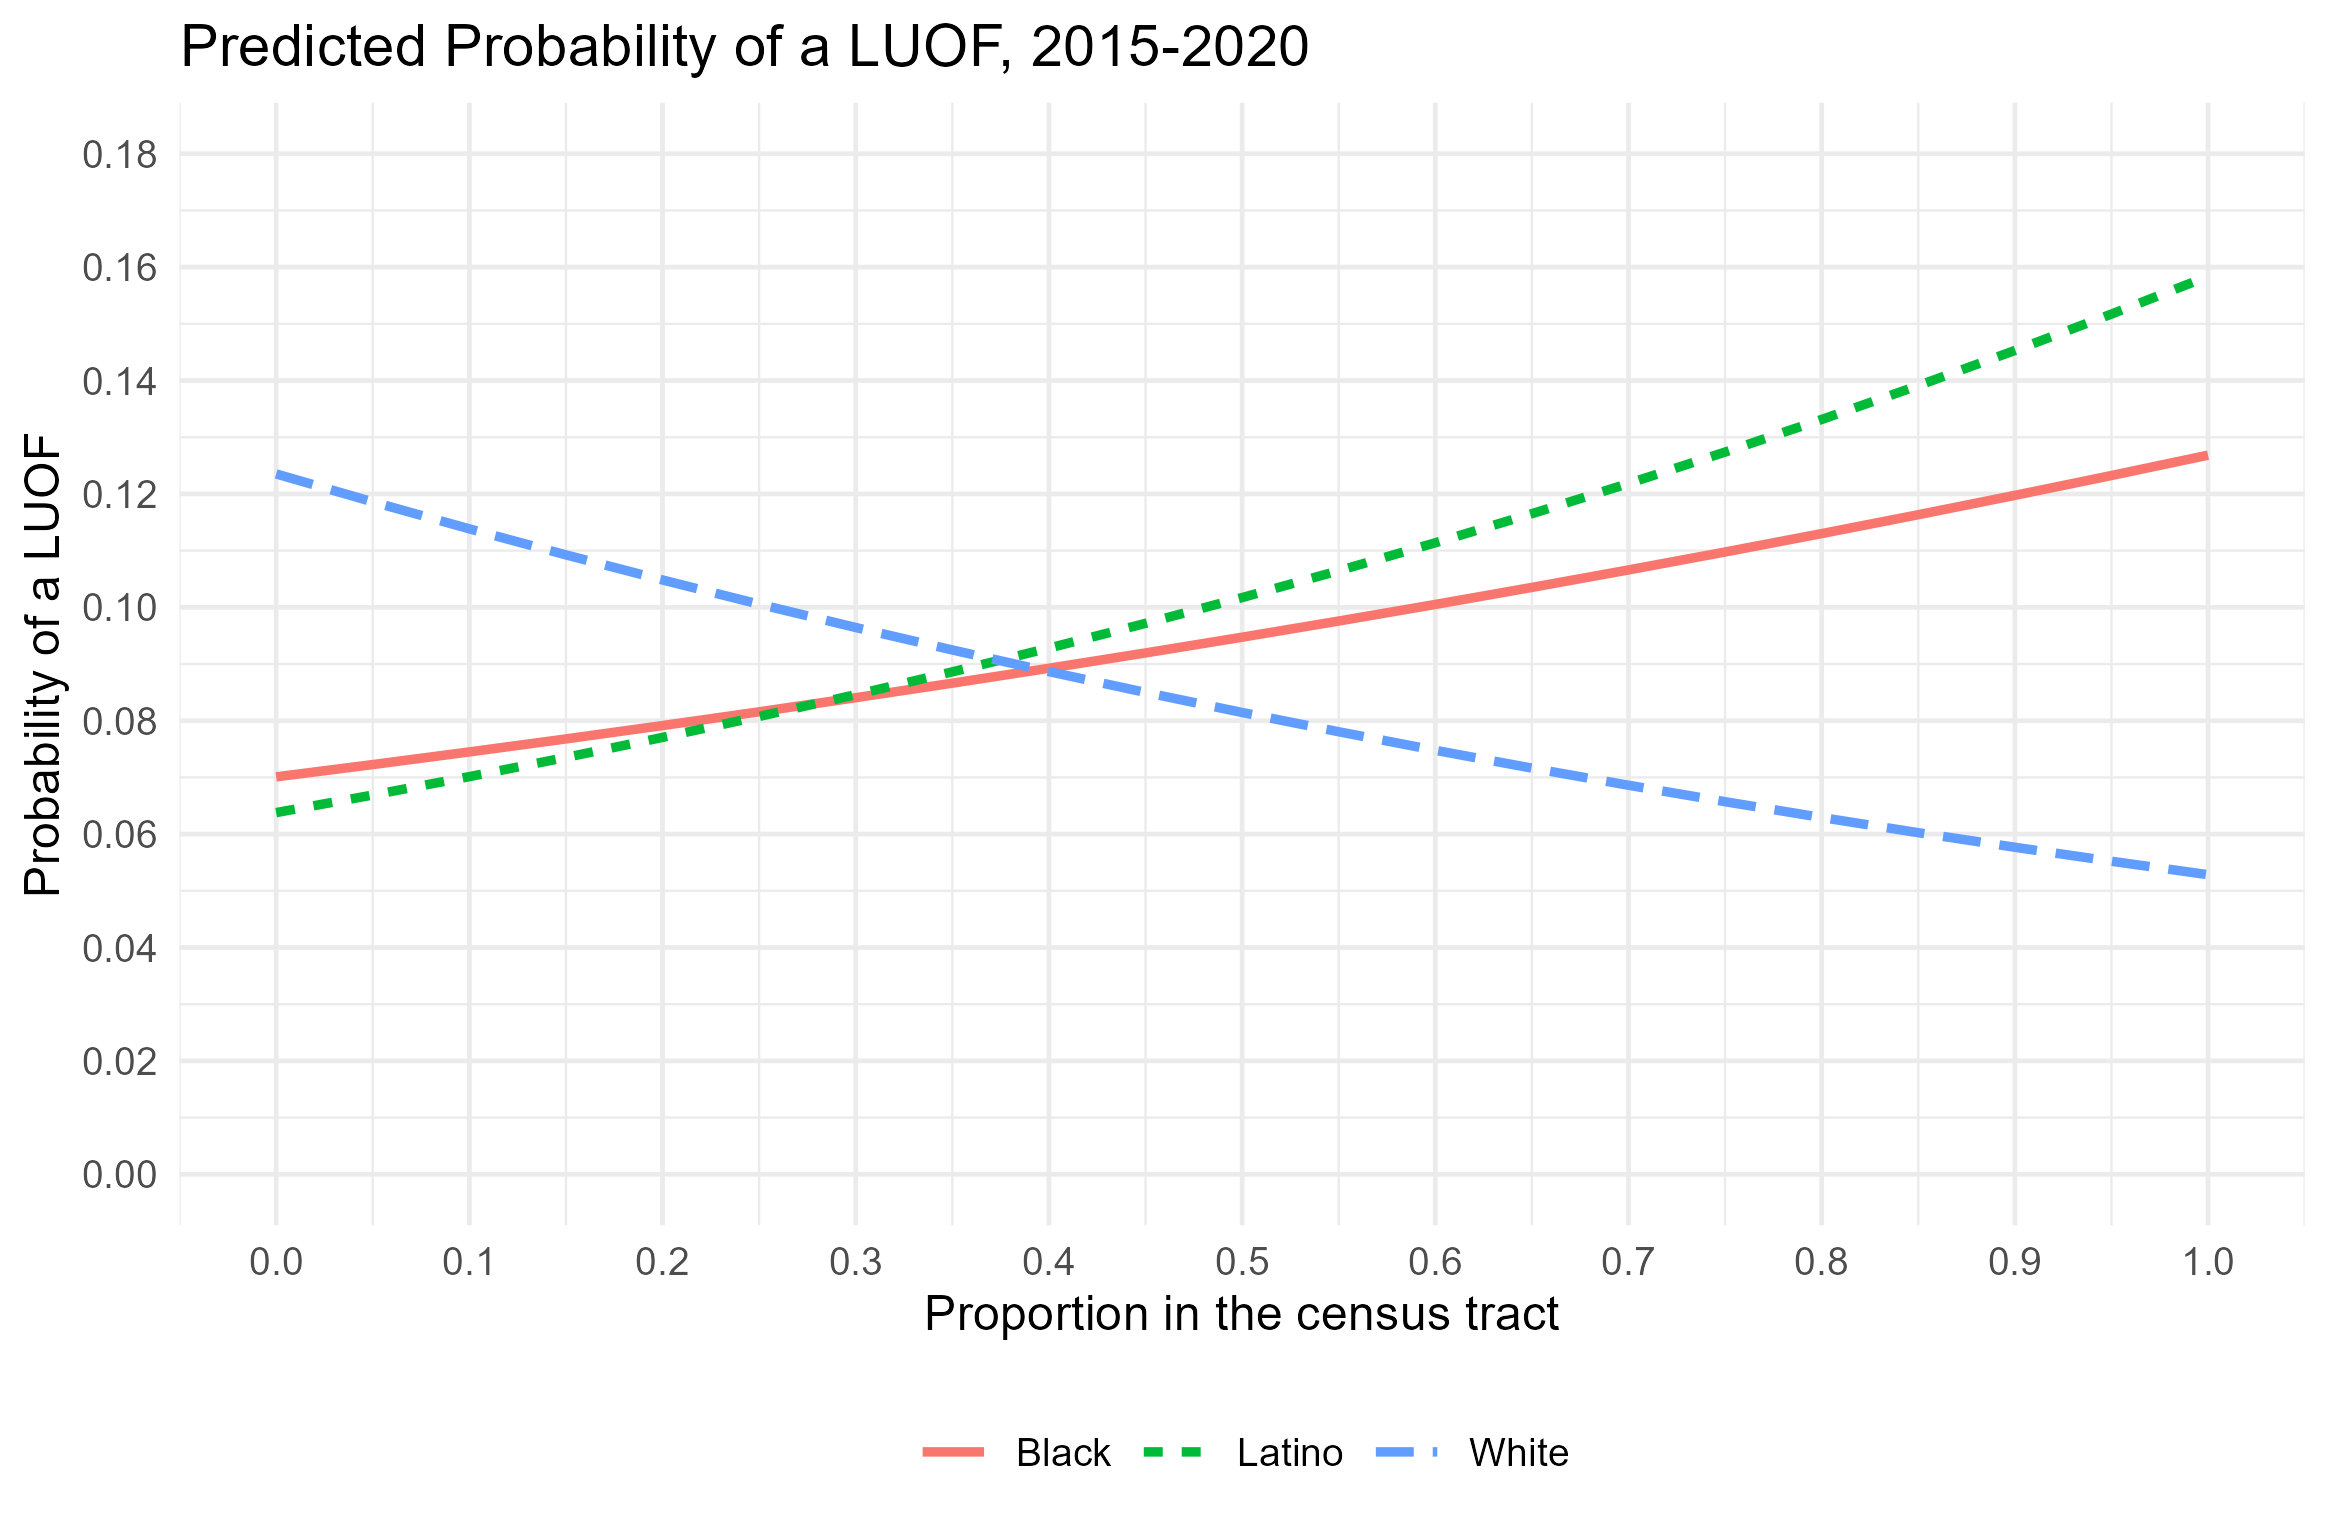
\includegraphics[width=\linewidth]{images/race_logit}
        \end{column}
        % Second column for the image
        \begin{column}{0.4\textwidth}
        	\resizebox{\linewidth}{!}{%
				\begin{tabular}{lrrcrrr}
                    \toprule
                    Dependent Var: & LUOF $\ge1$  & & & & & \\
                    \midrule
                    \midrule
                    Proportion & Coefficient & Std. err. & z & P$>|$z$|$ & \multicolumn{2}{c}{[95\% conf. interval]} \\
                    \midrule
                    Black 				& 0.655957 	& 0.055286 	& \text{ 11.86} 	& 0.000 	& 0.547598 	& 0.764316 \\
                    White 				& -0.926671 	& 0.041876 	&-22.13 				& 0.000 	& -1.008746 	& -0.844597 \\
                    Latino 			& 1.015783 	& 0.051397 	& \text{ 19.76} 	& 0.000 	& 0.915046 	& 1.116519 \\
                    \bottomrule
                \end{tabular}
			} \pause
			
			\vspace{20pt}
			
			Change in odds for every 0.10 in proportion:
			
			\vspace{10pt}
			
			Black: $e^{0.655957 \times 0.1} - 1 = 0.06779 \rightarrow 6.78$\%
			
			\vspace{10pt}
			
			White: $e^{-0.926671 \times 0.1} - 1 = -0.0885 \rightarrow -8.85$\%
			
			\vspace{10pt}
						
			Latino: $e^{1.015783 \times 0.1} - 1 = 0.1069 \rightarrow 10.69$\%
		\end{column}
	\end{columns}
	\note[item]{Regressions were also run to predict the odds of a LUOF based on what proportion of the tract was black, latino, and white.}
	\note<2>[item]{Again, we can estimate the effect of the racial proportions on the odds of the tract experiencing at least one LUOF.}
\end{frame}

\begin{frame}{Logistic Regressions: Marginal Effects}
	\begin{center}
		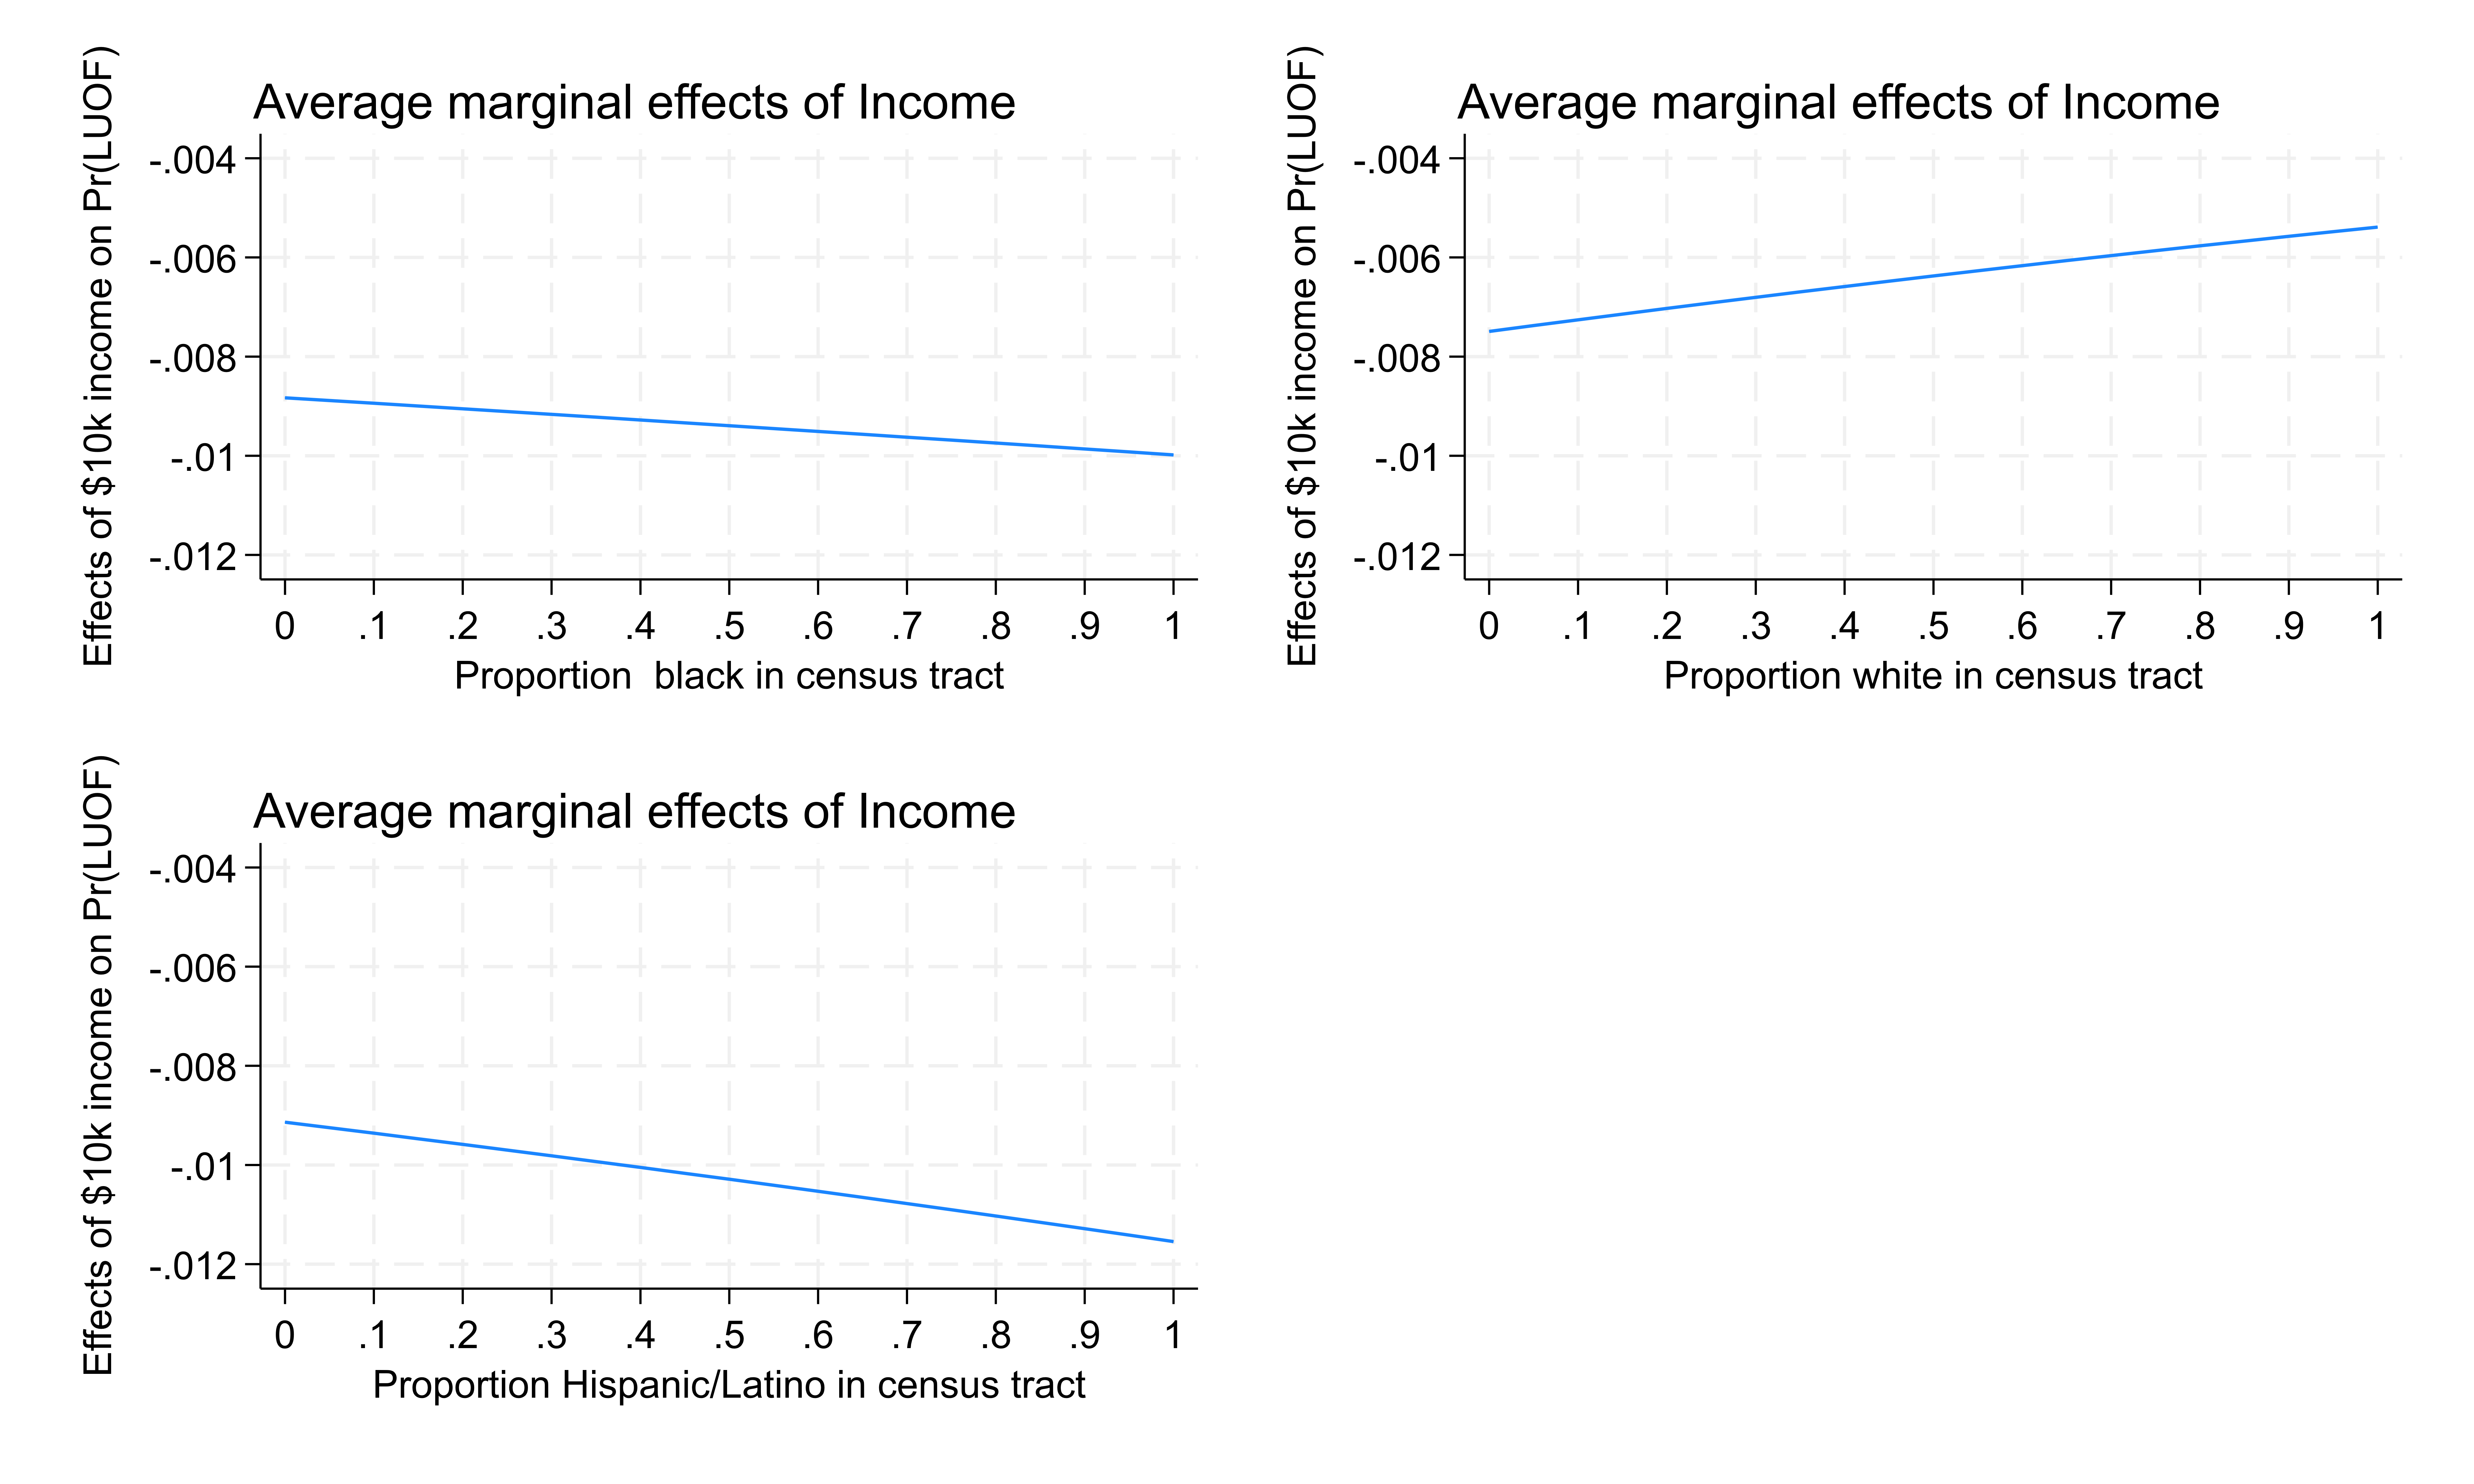
\includegraphics[height=0.85\textheight]{images/LUOF_logit_combined_effects}
	\end{center}
	\note[item]{Next, I ran the regressions with interactions between the racial proportions and median household income.}
	\note[item]{These plots show the average marginal effect of 10 thousand dollars income on the odds of the tract experiencing at least one LUOF at a given proportion.}
\end{frame}

%----- Gentrification -----%
\section{Findings: Gentrification}

\begin{frame}{Gentrification Typologies}
\begin{center}
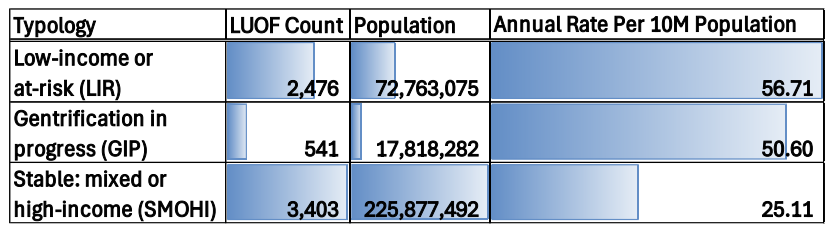
\includegraphics[width=0.75\linewidth]{images/udp_typology_only}
\end{center}
\end{frame}

\begin{frame}{Gentrification and Race}
	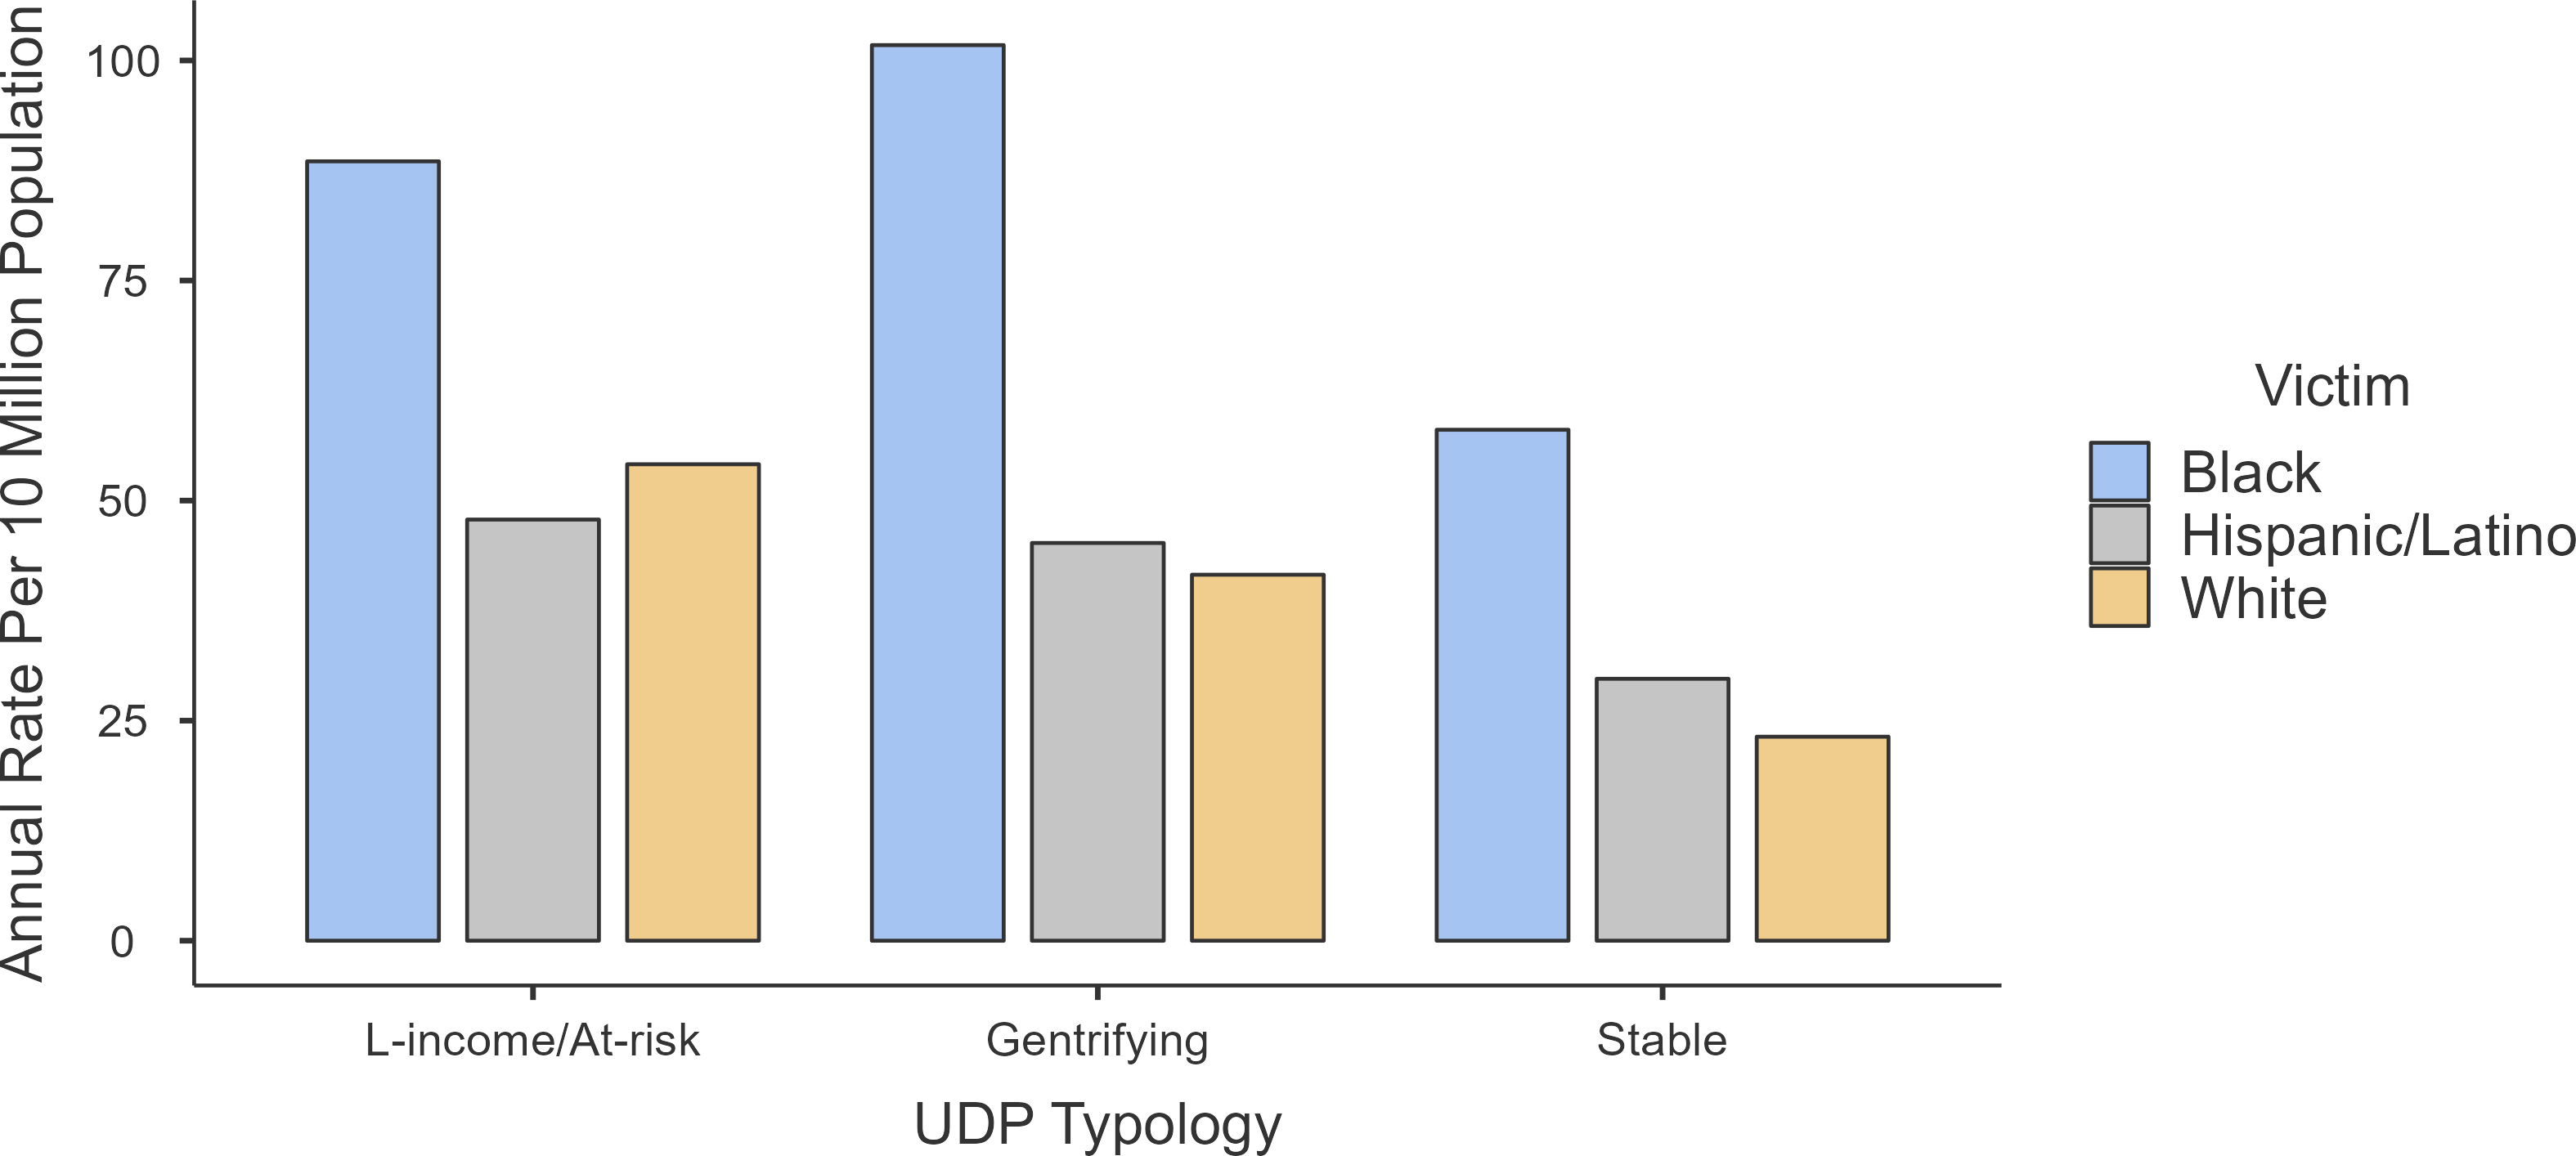
\includegraphics[width=0.49\linewidth]{images/udp_victim_race}
	\hfill
	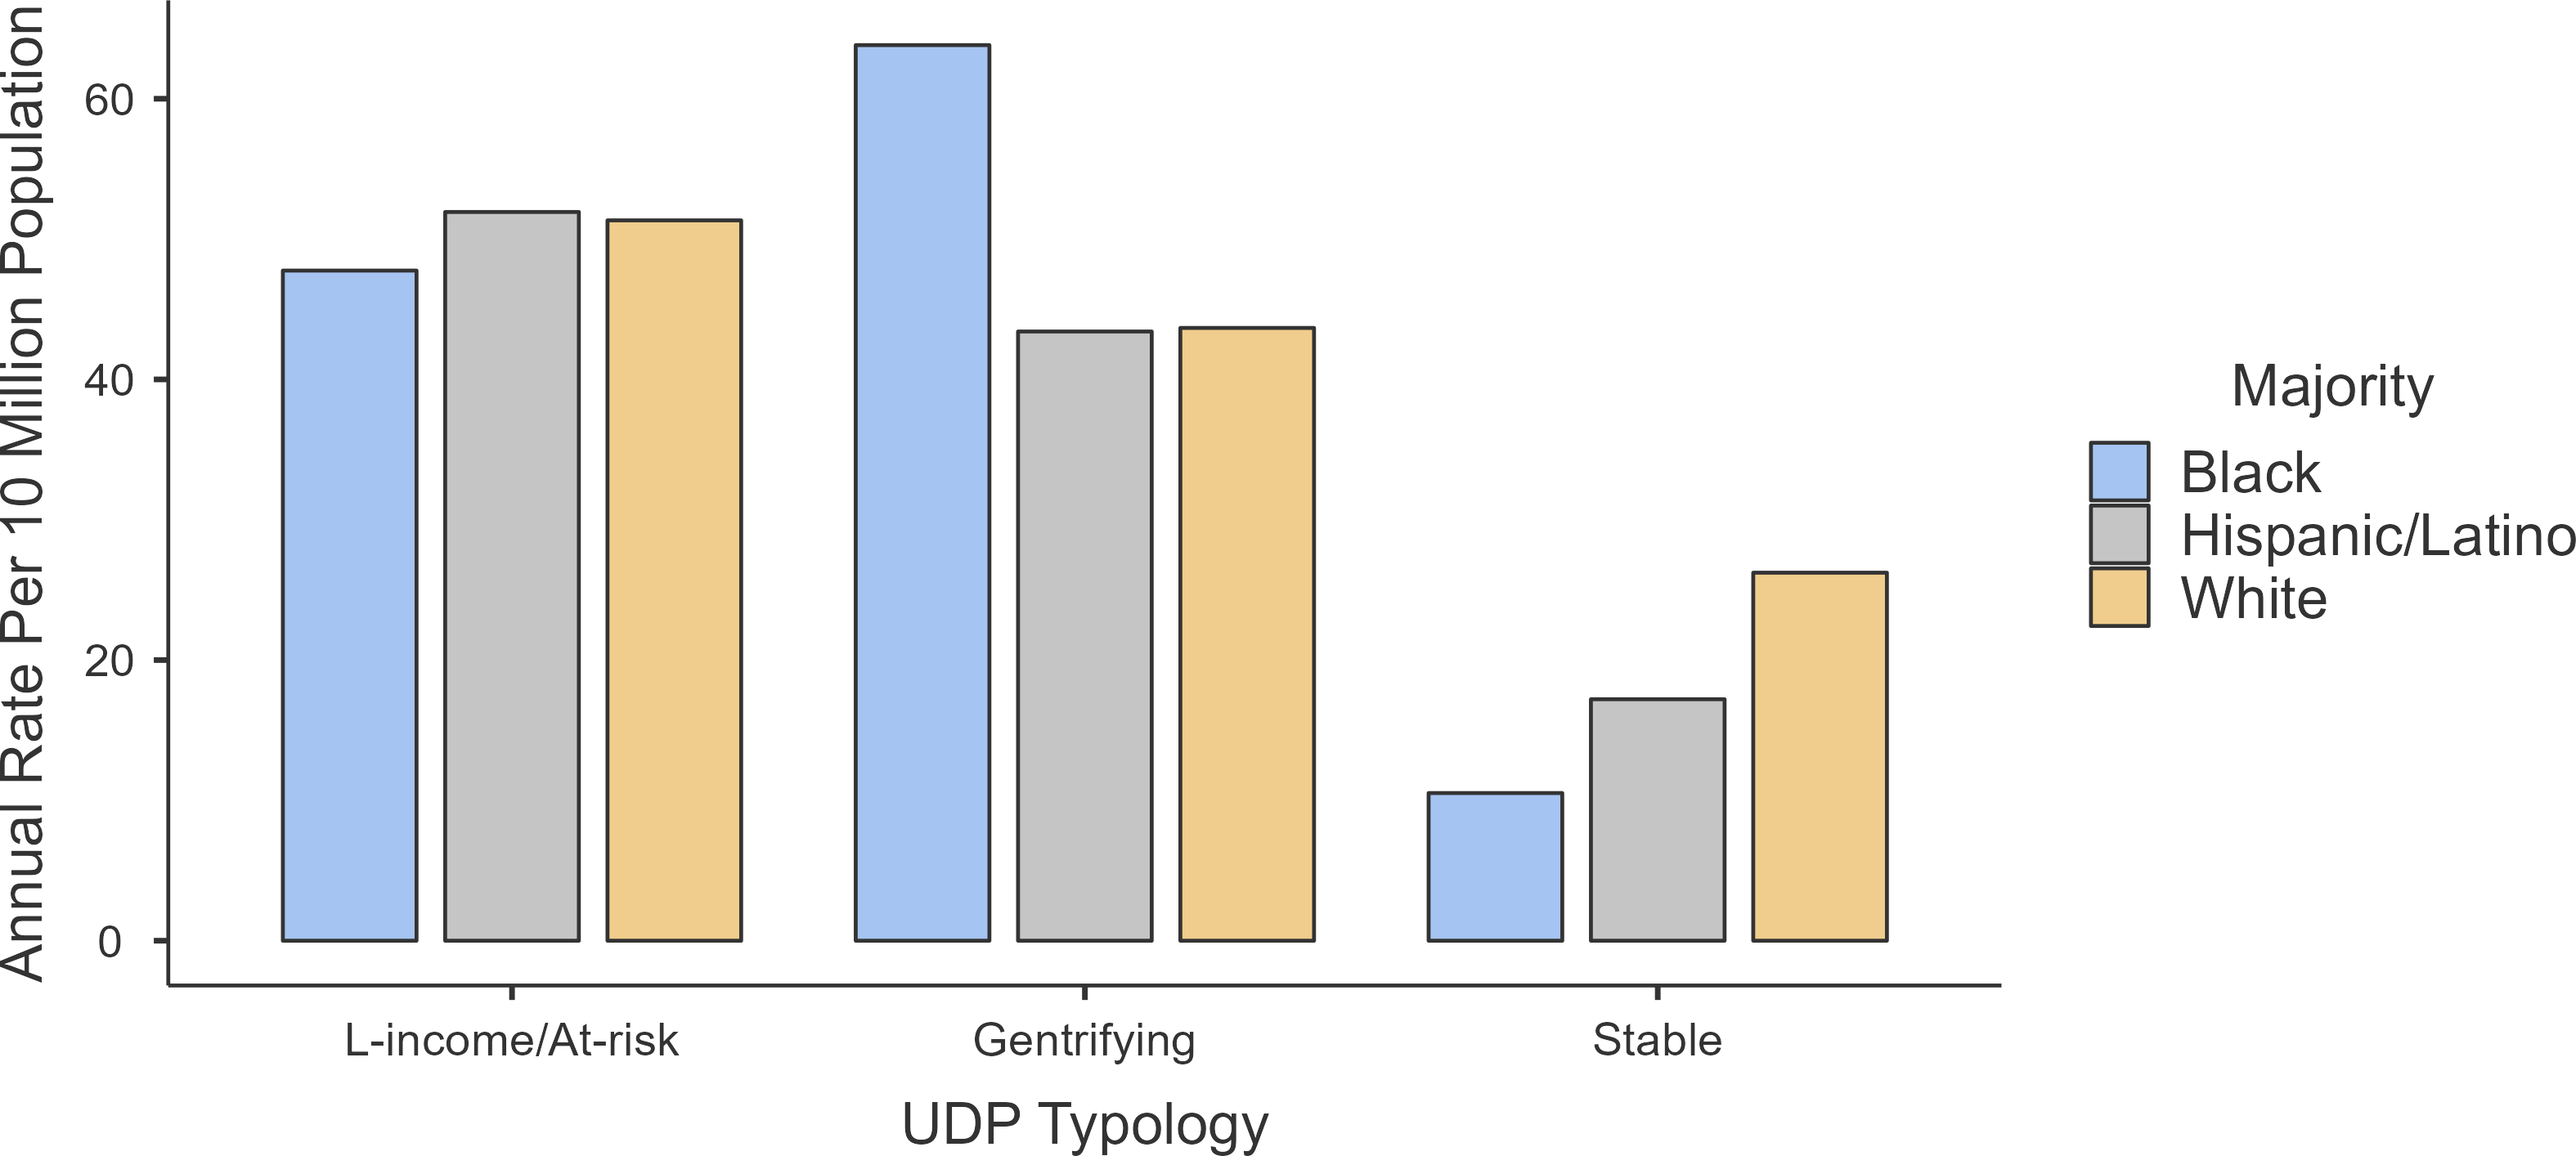
\includegraphics[width=0.49\linewidth]{images/udp_majority}
\end{frame}

\begin{frame}{Three Way Interaction: Gentrification, Majority Race \& Victim’s Race}
	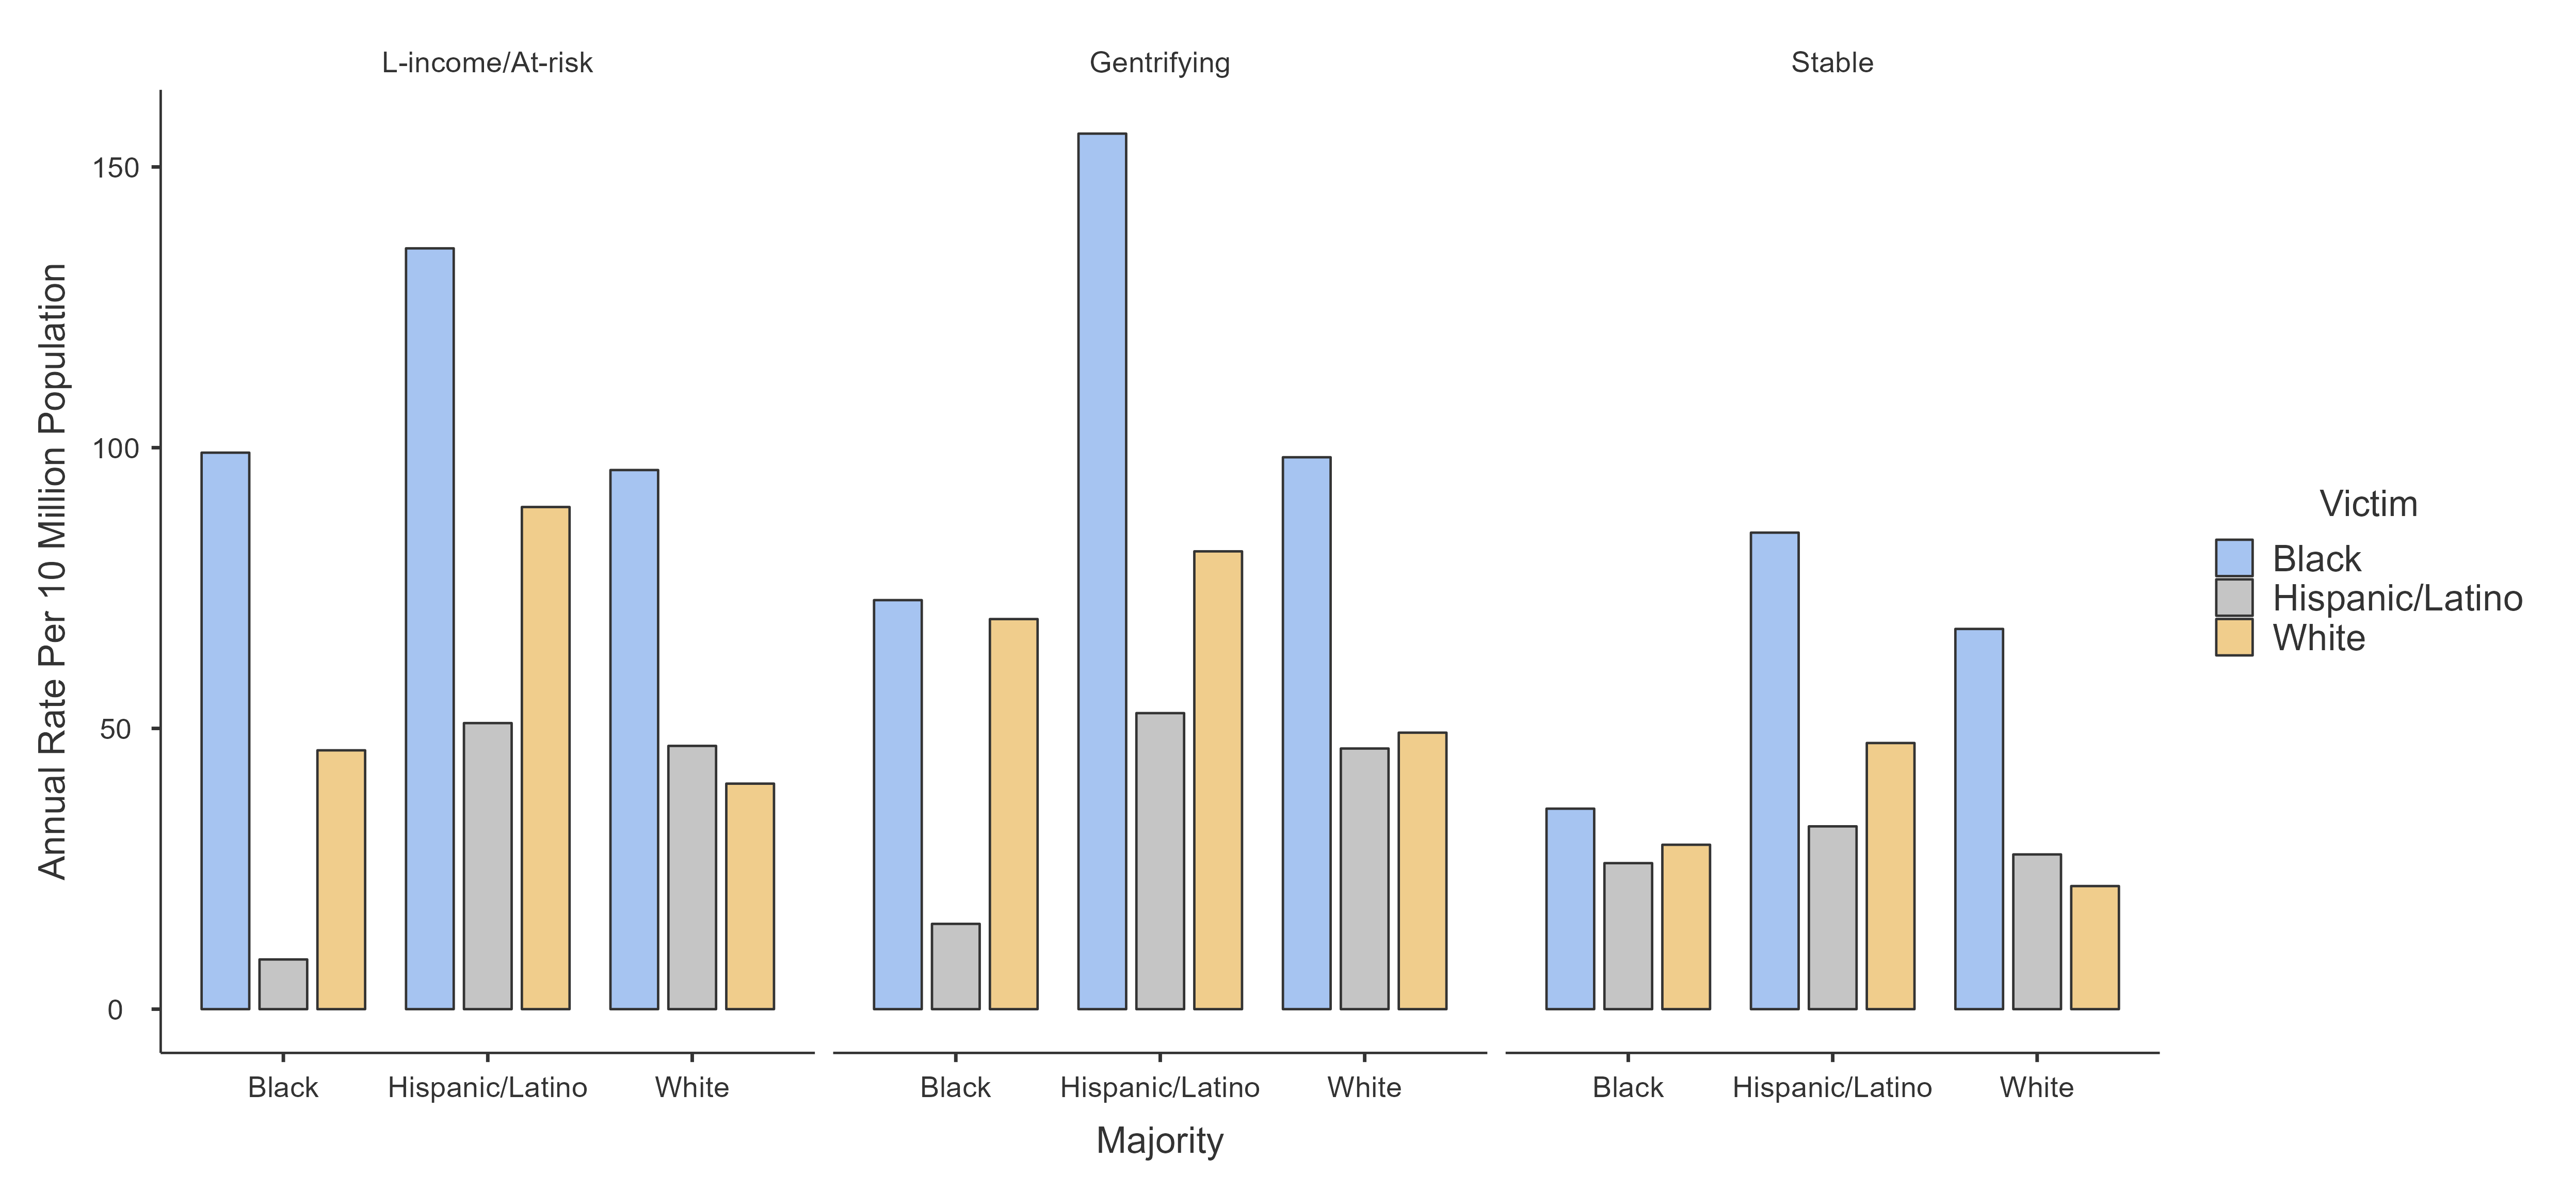
\includegraphics[width=\linewidth]{images/udp_race_majority_victim_legend}
\end{frame}

%\begin{frame}{Three Way Interaction: Gentrification, Majority Race \& Victim’s Race}
%	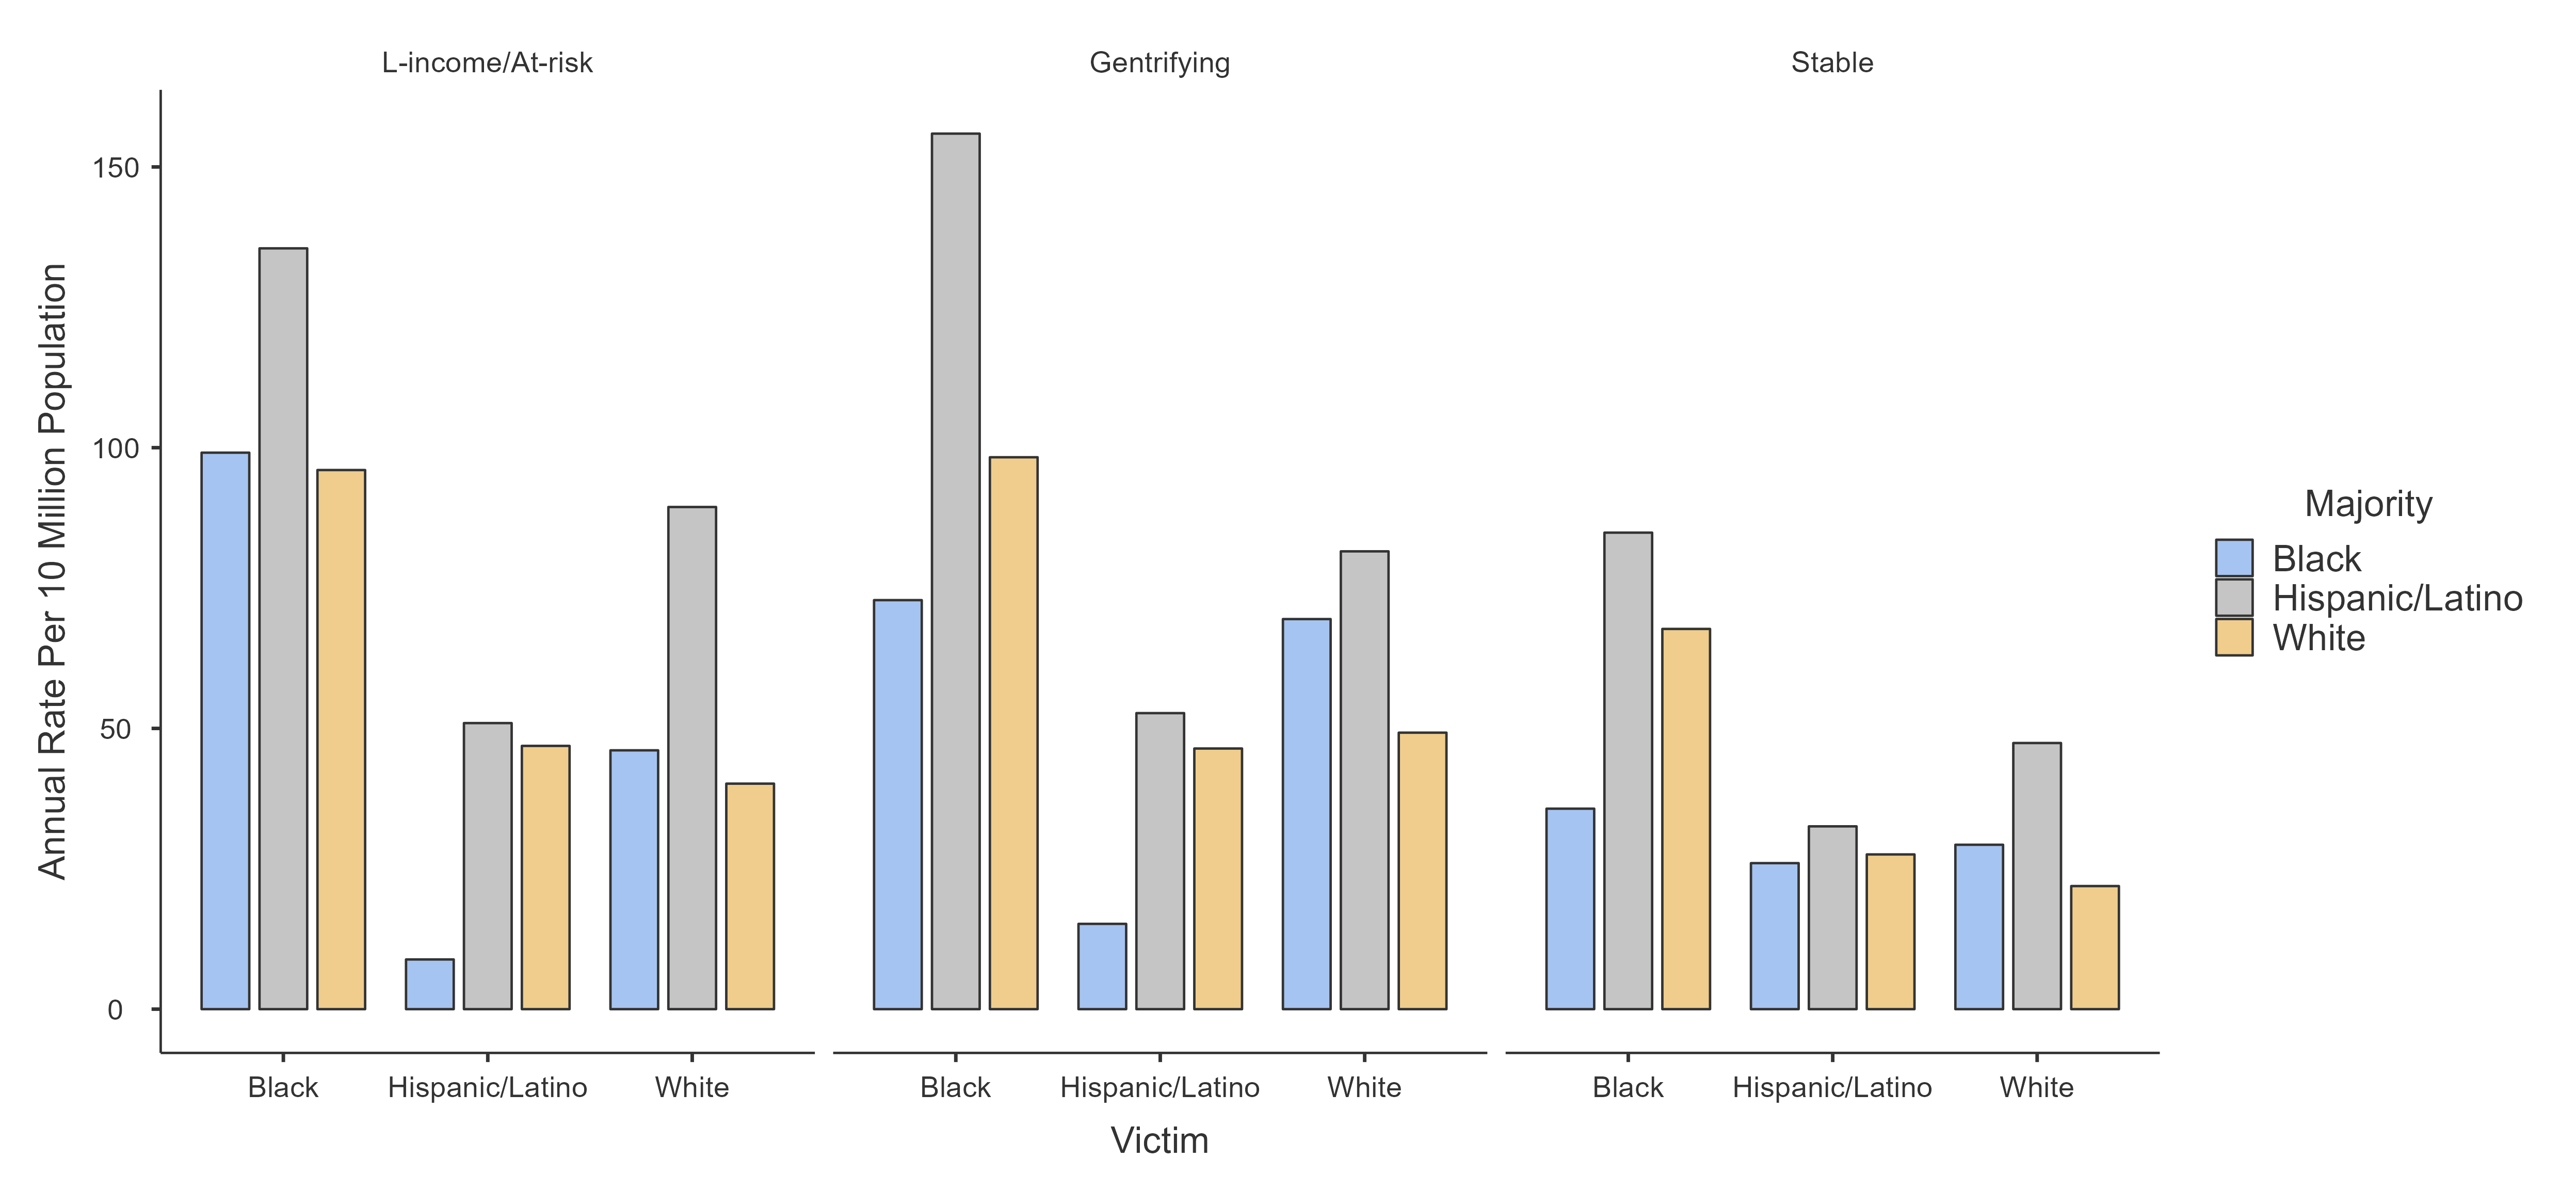
\includegraphics[width=\linewidth]{images/udp_victim_race_majority_legend}
%\end{frame}

%----- Discussion -----%
\section{Discussion}
\begin{frame}{Findings: Discussion}
	\begin{itemize}
	\item A clear relationship between median household income in census tracts where lethal uses of force (LUOFs) occurred.
	\item Though it would be a stretch to infer causality based strictly on these observational findings.
	\item Racial subordination needs to be understood in the context of economic relations and how those also contribute to the likelihood of a LUOF \parencite{johnsonAfterwordBaltimorePolicing2016, wacquantClassRaceHyperincarceration2010}.
	\item The relationship between the Urban Displacement Project’s typologies is unclear and inconclusive.
	\item Census tracts identified as gentrifying did not have higher LUOF rates compared to low-income/at-risk-of-displacement tracts.
	\item However, the rate for blacks in gentrifying tracts was higher.
	\end{itemize}
	\nocite{feldmanPoliceRelatedDeathsNeighborhood2019}
	\nocite{feldmanPoliceKillingsUS2020}
\end{frame}

%----- Limitations and Future Research -----%
%\begin{frame}{Limitations and Future Research}
%	Text goes here\ldots
%\end{frame}


%\begin{frame}
%                \begin{tabular}{lrrcrrr}
%                    \toprule
%                    Dependent Var: & LUOF $\ge1$  & & & & & \\
%                    \midrule
%                    \midrule
%                    Proportion & Coefficient & Std. err. & z & P$>|$z$|$ & \multicolumn{2}{c}{[95\% conf. interval]} \\
%                    \midrule
%                    Black 				& 0.655957 	& 0.055286 	& \text{ 11.86} 	& 0.000 	& 0.547598 	& 0.764316 \\
%                    White 				& -0.926671 	& 0.041876 	&-22.13 				& 0.000 	& -1.008746 	& -0.844597 \\
%                    Hisp/Latino 	& 1.015783 	& 0.051397 	& \text{ 19.76} 	& 0.000 	& 0.915046 	& 1.116519 \\
%                    \bottomrule
%                \end{tabular}
%\end{frame}

\sloppy
\begin{frame}{Bibliography}
%	\fontsize{4}{7.2}\selectfont
	\printbibliography
\end{frame}

%\begin{frame}{Racial Disparities}
%\begin{itemize}
%\begin{tabular}{|c|c|c|}
%  \hline
%  Header 1 & Header 2 & Header 3 \\
%  \hline
%  Row 1, Cell 1 & Row 1, Cell 2 & Row 1, Cell 3 \\
%  \hline
%  Row 2, Cell 1 & Row 2, Cell 2 & Row 2, Cell 3 \\
%  \hline
%\end{tabular}
%\end{itemize}
%\end{frame}

\end{document}